\documentclass[usenatbib,fleqn]{mn2e}
\usepackage{amsmath,amssymb}
\usepackage{graphicx}
\usepackage{epstopdf}
\epstopdfsetup{outdir=./figures/}
\graphicspath{{./figures/}}
\usepackage{url}
\usepackage{aas_macros}
\usepackage{astro}
% \usepackage{natbib}

% \renewcommand{\l}{\left}
% \renewcommand{\r}{\right}

\newcommand{\Mdot}{\dot{M}}
\newcommand{\eddr}{\dot{M}/\dot{M}_{\rm Edd}}
\newcommand{\Mdote}{\dot{M}_{\rm Edd}}
\newcommand{\Mdotb}{\dot{M}_{\rm bondi}}

\newcommand\lsim{\mathrel{\rlap{\lower4pt\hbox{\hskip1pt$\sim$}}
    \raise1pt\hbox{$<$}}}
\newcommand\gsim{\mathrel{\rlap{\lower4pt\hbox{\hskip1pt$\sim$}}
    \raise1pt\hbox{$>$}}}
\newcommand{\rs}{r_s}
\newcommand{\rb}{r_b}
\newcommand{\rcirc}{r_{\rm circ}}
\newcommand{\rss}{r_{\rm ss}}
\newcommand{\lrs}{\l_{\rs}}
\newcommand{\lambdars}{\lambda_{\rs}}
\newcommand{\vw}{v_w}

\newcommand{\dxdy}[2]{\frac{\partial #1}{\partial #2} }
\newcommand{\ddr}[1]{\dxdy{#1}{r}}
\newcommand{\drhodt}{\dxdy{\rho}{t}}
\newcommand{\dpdr}{\dxdy{p}{r}}
\newcommand{\dvdr}{\dxdy{v}{r}}
\newcommand{\dsdr}{\dxdy{s}{r}}
\newcommand{\dphidr}{\dxdy{\Phi}{r}}

\newcommand{\ke}{\frac{v^2}{2}}
\newcommand{\kew}{\frac{v_w^2}{2}}

\newcommand{\gammaf}{\frac{\gamma}{\gamma-1}}
\newcommand{\gammafi}{\frac{\gamma-1}{\gamma}}
\newcommand{\cs}{\frac{p}{\rho}}
\newcommand{\Q}{q (\ke+\kew-\gammaf \cs)}

\newcommand{\kb}{k_{\rm b}}
\renewcommand{\mp}{m_{\rm p}}
\newcommand{\pc}{\rm pc}

\newcommand{\Menc}{M_{\rm enc}}
\newcommand{\rhostar}{\rho_*}
\newcommand{\Mstar}{M_{\star}}
\newcommand{\Mseight}{M_{\star,8}}
\newcommand{\Mbh}[1][]{M_{\bullet#1}}
\newcommand{\Mbheight}{M_{\bullet,8}}
\newcommand{\MbheightExp}{\frac{\Mbh}{10^8 \Msun}}

\newcommand{\phirs}{\frac{G \Menc}{\rs}}
\newcommand{\soi}{\rm soi}
\newcommand{\rsoi}{r_{\soi}}
\newcommand{\ff}{\rm ff}
\newcommand{\tff}{t_{\ff}}
\newcommand{\rIa}{r_{\rm Ia}}
\newcommand{\EIa}{E_{\rm Ia}}
\newcommand{\RateIa}{R_{\rm Ia}}
\newcommand{\sigsoi}{\sigma_{\soi}}

\newcommand{\vwO}{v_{w,0}}
\newcommand{\kewO}{\frac{\vwO^2}{2}}
\newcommand{\x}{\frac{r_s}{\rsoi}}
\newcommand{\vwNorm}{\frac{\vwO}{\sigsoi}}
\newcommand{\vwOFH}{v_{w,0,500}}
\newcommand{\vwOFHexp}{\frac{\vwO}{500 \, {\rm km/s}}}

\newcommand{\pyear}{{\rm yr}^{-1}}
\newcommand{\tage}{t_{\star}}
\renewcommand{\th}{t_h}

\topmargin -1 cm
\defcitealias{WangMerritt:2004a}{WM04}	

\author[Generozov, Stone, \& Metzger]{Aleksey Generozov$\thanks{E-mail: ag@astro.columbia.edu}$, Nicholas Stone, Brian~D.~Metzger\\
  Columbia Astropysics Labratory, Columbia University, 550 West 120th Street, New York, NY 10027}


\begin{document}
\title{Modeling the Circumnuclear Mediums and Accetion Rates of Quiescent Supermassive Black Holes}
\maketitle

\begin{abstract}
  We calculate the steady-state hydrodynamic profiles of hot gas in
  the nuclei of a sample of early-type quiescent galaxies.  We assume
  that mass is supplied to the circumnuclear medium (CNM) entirely by
  stellar winds according to the radial stellar profiles for each
  galaxy, while the gas is heated by a combination of shocked stellar
  winds and supernovae.  Our analytic and numerical results are used
  to estimate the accretion rates onto the central supermassive black
  holes (SMBH) as a function of the SMBH mass $M_{\bullet}$ and the
  heating efficiency, the latter of which is related schematically to
  the age of the stellar population, the frequency of supernovae, and
  the efficacy of accretion feedback processes.  For a fixed heating
  efficiency, we find that the SMBH accretion Eddington factor
  increases with the SMBH mass, $\dot{M}/\dot{M}_{\rm edd} \propto
  M_{\bullet}^{\alpha}$ with $\alpha \approx 0.5, 1$ for cusp and core
  nuclei, respectively.
  % However, considering the potentially lower heating efficiency of low
  % mass SMBHs (due to a younger stellar population and the rareity of
  % supernovae within the stagnation radius) and their resulting higher
  % susceptibility to cooling instability, we find a flatter
  % relationship $\alpha \approx 0$. 
  Our results are used to check previous estimates of the SMBH
  accretion rate assuming Bondi accretion and extrapolating the X-ray
  measured density and temperature to the unresolved Bondi radius.  We
  also discuss the implications of our results for the diversity of
  CNM environments encountered by the jetted outflows from tidal
  disruption events, and for the use of an assumed
  $\dot{M}-M_{\bullet}$ relationship to constrain the occupation
  fraction of SMBHs in low mass galaxies.
\end{abstract}

\begin{keywords}
  black hole physics --  galaxies: active
\end{keywords}


\section{Introduction}
\label{sec:introduction}

%% Maybe active galaxies constitute 10% need reference here?
Supermassive black holes (SMBHs) lurk in the centers of most, if not
all nearby galaxies (see reviews by,
e.g. \citealt{KormendyRichstone:1995a};
\citealt{FerrareseFord:2005a}). However, only a few percent of these
manifest themselves as luminous Active Galactic Nuclei (AGN).  Nearly
quiescent SMBHs, such as those hosting low luminosity AGN, constitute
a silent majority (e.g.~\citealt{Ho:2009a}).

In order to understand why most SMBHs appear to be inactive, it is
necessary to understand their gaseous environments.  Hot gas near the
SMBH sphere of influence (the `circumnuclear medium' or CNM) controls
the central mass accretion rate $\dot{M}$.  Better knowledge of how
$\dot{M}$ varies with the SMBH mass $\Mbh$ and other properties of the
galactic nucleus is necessary to understand the co-evolution of SMBHs
and their host galaxies with cosmic time.  SMBH growth in the low
redshift universe, for instance, appears to be dominated by low mass
black holes (e.g.~\citealt{Heckman+04}).  Although this is often
attributed to cosmological ``down sizing" (e.g, \citealt{Gallo+08}),
the physical processes involved may be distinct from those operating
at higher SMBH masses and accretion rates in quasars.

The accretion rates of low mass SMBHs and their resulting nuclear
X-ray luminosities $L_X$ also have implications for observational
constraints on their occupation fraction in low mass galaxies and the
possible existence of intermediate mass black holes.
\citet{MillerGallo+:2014a} combine the relationship between $\Mbh$ and
$L_X$ from a sample of relatively high mass galaxies
(\citealt{Gallo+08}) with upper limits on $L_X$ in several lower mass
galaxies, to infer tentative evidence for an occupation fraction less
than unity.  However, this method relies on extrapolating a power-law
fit to the $L_X-\Mbh$ distribution to low $\Mbh$, below the
instrumental detection threshold.  The conclusions of
\citet{MillerGallo+:2014a} are thus sensitive to possible changes in
the $L_X$-$\Mbh$ relationship at small $\Mbh$.
% AG: In our model we obtain a steeper relationship, but we have difficulty matching the observed relationship above the detection threshold

The density profile of the CNM also influences the emission from
stellar tidal disruption events (TDEs), such as the high energy
transient {\it Swift} J1644+57 (\citealt{Levan+11};
\citealt{Bloom+11}, \citealt{Burrows+11}; \citealt{Zauderer+11}).
This event was powered by a transient relativistic jet, which produced
synchrotron radio emission as the jet material was decelerated by
shock interaction with the CNM of the previously quiescent SMBH
(\citealt{Giannios&Metzger11}; \citealt{Zauderer+11}).  Detailed
modeling of {\it Swift} J1644+57 showed that the CNM density was
significantly lower than that measured surrounding Sgr A$^{\star}$
(\citealt{Metzger+12}; \citealt{Berger+12}).  However, a TDE jet
injected into a denser CNM would be decelerated more rapidly,
producing substantially different radio emission than in {\it Swift}
J1644+57.  Variations in the properties of the CNM could thus in
principle help explain why most TDEs appear to be radio quiet
(e.g.~\citealt{Bower+13}; \citealt{VanVelzen+13}).

Gas that forms the CNM of a SMBH may originate from several sources
(\citealt{Ho:2009a}): (1) wind mass loss from (predominantly evolved)
stars; (2) star-star collisions; (3) the unbound debris from TDEs.
Stellar wind mass loss is probably the dominant source in most cases
insofar as collisions are relevant only in very dense stellar
environments for young stellar populations (\citealt{Rubin&Loeb11}),
while TDEs are estimated to provide a subdominant contribution to the
time-averaged accretion rate of quiescent SMBHs
(\citealt{MacLeod+13}).

\citet{Ho:2009a} calculates the accretion rates onto a sample of
early-type galaxies both by using X-ray observations to determine the
Bondi accretion rate, and by estimating the contributions from the
mass loss of evolved stars.  Both methods lead him to conclude that
the available reservoir of gas is more than sufficient to power
low-luminosity AGN, assuming the standard radiative efficiency $\eta
\sim 0.1$ for thin disk accretion.  Indeed, there is now strong
observational evidence that the low levels of AGN activity in
quiescent galaxies results from accretion proceeding in a radiatively
inefficient mode (\citealt{Yuan&Narayan14}), either due to the
gravitationally-released energy being advected across the SMBH horizon
(e.g.~\citealt{Narayan&Yi95}) or due to only a fraction of the gas
inflowing on large scales ultimately reaching the SMBH
(e.g.~\citealt{Blandford&Begelman99}; \citealt{Li+13}).

The accretion rates of SMBHs can in principle be estimated directly by
assuming Bondi accretion and using {\it Chandra} X-ray observations to
estimate the gas temperature and density near the Bondi radius.  This
technique has led to the intriguing result that the Bondi accretion
power correlates with the AGN jet power (e.g.,
\citealt{AllenDunn+:2006a}; \citealt{Russell+13};
\citealt{FujitaKawakatu+:2014a}), the latter estimated from the energy
required to inflate the observed cavities within the X-ray emitting
gas.  It is, however, almost never possible to resolve the Bondi
radius, thus requiring all such studies to extrapolate the observed
gas temperature and density profiles to much smaller radial scales.
%In fact, the temperature profile is assumed to be flat inside of the
%Bondi radius.  In reality, the cusp in the velocity dispersion near
%the SMBH, should cause a cusp in the gas temperature profile (assuming
%the kinetic energy of stellar winds is efficiently thermalized in
%shocks).
%% AG-give sense of scale.

Another approach to determine the SMBH accretion rate, which we adopt
in this paper, is to directly calculate the density, velocity and
temperature profiles of the CNM using a physically motivated
hydrodynamic model.  Mass is injected to the nuclear environment via
stellar winds, while energy input results from a number of sources,
such as wind shock heating and supernovae (e.g.,
\citealt{Quataert:2004a,De-ColleGuillochon+:2012a,ShcherbakovWong+:2014a}).
Unlike previous works, however, which focus on modeling the nuclei of
individual galaxies, here we systematically analyze the properties of
the CNM across a large sample of quiescent galaxies with a range of
SMBH masses and other properties (\citealt{WangMerritt:2004a};
hereafter WM04).  For each galaxy, stellar winds deposit mass and
energy across a range of radii calculated directly from the observed
{\it stellar} density profile.

The one-dimensional steady state flow of gas is usually characterized
by an inflow-outflow structure, with a critical radius known as the
``stagnation radius" $\rs$ where the radial velocity goes to zero.
Mass loss from stars interior to the stagnation radius is accreted,
while that outside $\rs$ is unbound in an outflow from the nucleus.
The stagnation radius, rather than the Bondi radius, is thus
ultimately responsible for setting the SMBH accretion rate, although
$\rs$ can in many cases lie within a factor of few of the
nominal Bondi radius.
% Furthermore, in some cases we find that no stagnation
% radius exists at all; this formally implies that the entire of ISM of
% the galaxy is feeding the SMBH, potentially resulting in much higher
% accretion rate than would be predicted by simple Bondi accretion. 
The main goal of our analysis is to provide a framework for
interpreting the properties of quiescent galactic nuclei given the
comparatively well understood physics of stellar winds and supernova
heating.

This paper is organized as followed.  In $\S\ref{sec:model}$ we
describe our model, including the sample of galaxies used in our
analysis ($\S\ref{sec:sample}$) and our numerical procedure for
calculating the steady-state hydrodynamic profile of the CNM
($\S\ref{sec:hydro}$).  In $\S\ref{sec:results}$ we describe our
results.  In $\S\ref{sec:applications}$ we describe applicaiton of our
results, including a comparison of our gas profiles to those inferred
from {\it Chandra} observations and to the measured $L_X-\Mbh$
relationship.  In $\S\ref{sec:discussion}$ we discuss our results.  In
$\S\ref{sec:summary}$ we summarize our results.
\section{Model}
\label{sec:model}

\subsection{Galaxy Sample}

\label{sec:sample}

Our sample includes 61 early-type galaxies from \citetalias{WangMerritt:2004a}, as represent a subset of a larger sample of \citet{FaberTremaine+:1997a} with Hubble WFPC2 imaging.  We focus on elliptical galaxies because we are interested in isolating SMBHs fed by the steady mass loss from the relatively old stellar population, instead of fresh gas flowing into the sphere of influence from larger scales.

The surface brightness of each galaxy in the sample is parameterized by a Nuker Law (WM04; their Table 1),
\begin{equation}
  I(\xi)=I_b 2^{(\beta-\Gamma)/\alpha} \xi^{-\Gamma} (1+\xi^\alpha)^{-(\beta-\Gamma)/\alpha}, \,\,\,\xi\equiv\frac{r}{r_b}.
\end{equation}
The Nuker profile is a broken power law which transitions from an inner power law slope, $\Gamma$, to an outer power law slope, $\beta$, at a break radius, $\rb$.  

Given $I(\xi)$ we follow the procedure outlined by
\citetalias{WangMerritt:2004a} to compute the spherically-symmetric
stellar density profile $\rhostar(r)$ and stellar mass profile
$M_{\star}(r) = 4\pi \int \rhostar r^{2}dr$, both of which are used in
our model.  For reference, note that stellar density $\rhostar\sim
r^{-1-\Gamma}$ for $r \ll \rb$ and $\rhostar\sim r^{-1-\beta}$ for $r
\gg \rb$.  Since $\Gamma\approx 1$ for ``cusp" galaxies, while
$\Gamma\approx 0$ for ``core" galaxies, at small radii $\ll \rb$ we
thus have $\rhostar \propto r^{-\alpha}$ and $M_{\star} \propto
r^{\beta}$ with $\beta = 3-\alpha \approx 1-2$.  For each galaxy the
SMBH mass $\Mbh$ is determined from the $\Mbh-\sigma$ relationship.
%%AG-ugh I just took the Mbh from Wang & Merritt, which I guess is
%%calculated from an outdated M-sigma. It would be bizarre to use 2
%%different relations.


% AG:Is there a systematic dependence of beta on galaxy type$.

%% AG--some discussion of alternate parameterizations.  My intuition
%% is that for our purposes the parameterization should not
%% matter. But some discussion of alternate possibilities could
%% prevent Alistar Graham from yelling at us.

\subsection{Hydrodynamic Equations}
\label{sec:hydro}

Following \citet{Quataert:2004a} (see also \citealt{HolzerAxford:1970a,De-ColleGuillochon+:2012a,ShcherbakovWong+:2014a}), we calculate the gas density profile $\rho$ of the CNM for each galaxy within our sample by solving the equations of one-dimensional (spherically symmetric) time-dependent hydrodynamics,
\begin{align}
  &\drhodt+\frac{1}{r^2}\frac{\partial}{\partial r}\left(\rho r^2 v\right)=q \label{eq:drhodt}\\
  &\rho \left(\frac{\partial v}{\partial t} + v\frac{\partial v}{\partial r}\right) =-\dpdr- \rho\frac{GM_{\bf enc}}{r^{2}} -q v \label{eq:dvdt}\\
  &\rho T\left(\frac{\partial s}{\partial t} + v\frac{\partial
      s}{\partial r}\right)=q\left[\ke+\kew-\gammaf \cs \right] +\nabla\cdot(\kappa \nabla T)
, 
\label{eq:dsdt}
\end{align}
where $v$, $T$, $p$ and $s$ are the radial velocity, temperature,
pressure and specific entropy of the gas, respectively, and $M_{\rm enc} = M_{\star}(r) + \Mbh$ is the
enclosed mass.  We assume an ideal gas equation of state with $p =
\rho kT/\mu m_p$ with $\mu = 0.62$  and $\gamma = 5/3$. {\bf BDM: take $\mu = 0.62$ here for fully ionized gas}

The source term in the continuity equation (equation~\ref{eq:drhodt}),
%Should equations be referenced as equation of equation
\begin{align}
  q=\frac{\eta \rhostar}{\th},
\label{eq:q}
\end{align}
represents mass input from stellar winds, which we parameterize in
terms of the fraction $\eta$ of the stellar density $\rhostar$ being
recycled into gas on the Hubble time $\th = 10^{10}$ years (see, e.g.,
\citealt{Ciotti+91}).  In Appendix \ref{app:eta} we estimate that
$\eta \approx 0.11(t_{\star}/t_{\rm h})^{-1.26}$ for a Salpeter IMF,
assuming that all stars are formed in a burst of star formation at a
common age of $t_{\star}$ (equation~[\ref{eq:eta}]).  We adopt
$\eta=0.1$ as fiducial {\bf BDM: take $\eta = 0.1$ instead of 1}, but note that changing $\eta$ is equivalent to
rescaling $\rho$ by the same factor.\footnote{This is {\it not} true
  if cooling is included, since the cooling rate is proportional to
  density {\it squared}.}

Source terms $\propto q$ also appear in the momentum and entropy
equations (equation~[\ref{eq:dvdt}] and [\ref{eq:dsdt}]) due to the fact
that the isotropic mass injection in the rest frame of the SMBH
represents a source of momentum and energy relative to the mean flow (see also below).  
%No net momentum is in the winds, but mass is being added which adds a
%term in the velocity equation...

The second source term in equation (\ref{eq:dsdt}) accounts for heating transportation by electron conductivity, where the conductivity $\kappa = \kappa_0 T^{5/2}$ is assumed to equal the classical ``Spitzer" value (\citealt{Spitzer62}); although even a weak magnetic field could in principle strongly suppress the conductivity perpendicular to the field, the radially-decreasing temperature profiles of interest are susceptible to the magneto-thermal instability (\citealt{Balbus01}), the non-linear evolution of which is believed to result in a radially-directed field structure (\citealt{Parrish&Stone07}).

Following \citet{ShcherbakovWong+:2014a}, the term in the entropy
equation $\propto \vw^2 = \sigma(r)^2+v_{w,0}^2$ accounts for external
heating sources.  Here $\sigma(r) = \sqrt{GM_{\rm enc}/r}$ is the
velocity dispersion of the stars, thus accounting for the fact that at
a minimum the gas experiences shock heating between the stellar winds
of velocities moving with respect to each other a characteristic
velocity $\sim \sigma$.  This heating is present if the wind velocities themselves
are low, $\ll \sigma$, as characterize the majority of AGB mass loss.
The term $v_{w,0}^{2}$ parameterizes additional sources of heating,
such as main sequence winds, millisecond pulsars, supernovae, etc.  As
discussed in $\S\ref{sec:heating}$, the value of $v_{w,0}$ is
uncertain and will in general depend on the SMBH mass and the age of
the stellar population.

Equations (\ref{eq:drhodt})-(\ref{eq:dsdt}) are solved using a sixth
order finite difference scheme with a third order Runge-Kutta scheme
for time integration and artificial viscosity terms in the velocity
and entropy equations for numerical stability (\citealt{Brandenburg:2003a}).  We solve the equations for
different choices of $v_{\rm w,0}$ spanning the physically expected
range.  Although we are most interested in the steady-state CNM
structure, the time-dependent equations are solved to avoid numerical
issues that arise near the critical sonic points, of which there are
up to two because of the supersonic inflow on small radial scales and
a possible supersonic outflow on large scales.

We do not include radiative cooling in the entropy equation because
across much of the parameter space radiative cooling is negligible
compared to other sources of cooling (e.g., advection).  Although radiative
cooling cannot be neglected in some cases (especially if $\vwO$ is low
or $\eta$ is high), our 1D scheme cannot account for the true multi-phase behavior of local thermal instabilities anyways (e.g.~\citealt{textit}).  Our steady state solutions neglecting radiation can
nevertheless be used to ascertain over what parameter space cooling
instabilities are likely to develop ($\S\ref{sec:cooling}$).
%Dependence of the heating to cooling ratio has a far steeper
%dependence on vwO than on eta...

The accuracy of our numerical solutions is assessed by checking the
level of conservation of mass across the grid, as well as the integral
constraint on the energy.  Mass and energy are conserved to $\lesssim
40$ per cent for all solutions presented in this
paper. 
{\bf BDM: more details...}


\section{Results}

We begin by describing a number of useful analytic results before describing our numerical solutions.  

\label{sec:results}
\subsection{Analytics: Flow properties at $\rs$}

This section summarizes analytic estimates of several physical quantities of interest, such as the stagnation radius $\rs$ and the mass accretion rate, the detailed derivation of which are given in Appendix \ref{app:rs}.  All of our results are derived under the assumption that thermal conductivity can be neglected.

When possible our results are expressed in terms of the wind heating
parameter $v_{\rm w,0}$; the power-law slope of the density profile
$n$ (also evaluated at $r = \rs$); and the dimensionless parameter \be
\chi \equiv v_{\rm w}^{2}/v_{\rm w,0}^{2} \approx \left(1 + \sigma^{2}/v_{\rm w,0}^{2}\right) \approx
\left(1+0.14 \Mbheight^{0.43}v_{500}^{-1}\right), \ee where $v_{500}
\equiv v_{w,0}/500$ km s$^{-1}$, $M_{\bullet,8} \equiv
M_{\bullet}/10^{8}M_{\odot}$, and the second equality makes use of the
$M_{\bullet}-\sigma$ correlation (\citealt{Gultekin+09}) \be
M_{\bullet} \simeq 2\times 10^{8}\left(\frac{\sigma}{200\,{\rm
      km\,s^{-1}}}\right)^{5.1}M_{\odot}.
\label{eq:Msigma}
\ee
Although the use of equation (\ref{eq:Msigma}) is questionable for low mass BHs (e.g., \citealt{Greene&Ho07}), our results are not particularly sensitive to this assumption.  

First, by demanding continuity of the entropy derivative at the stagnation radius, the temperature at the stagnation radius is given by.
\begin{align}
T \simeq \frac{\gamma-1}{\gamma}\frac{\mu m_p v_{w}^{2}}{2} \approx 3.7
\times 10^6\,\chi v_{500}^2 \,\,{\rm K} 
\label{eq:Tanalytic}
\end{align}
%{\bf BDM: i picked $\mu = 0.62$ and stick to it.}

Demanding hydrostatic equilibrium at the stagnation point provides an expression for the stagnation radius
\begin{align}
  \x=\frac{1}{\zeta^2 n}\left[
    \frac{\Mstar}{\Mbh}\left(A-\frac{n}{2}\right)+(B-\frac{n}{2})\right],
  \label{eq:stag_analytic}
\end{align}
where $\zeta \equiv v_{w,0}/\sigma$, $n$ is the power-law slope of the
density profile at $r = r_{\rm s}$,

\begin{align}
r_{\rm soi} = \frac{GM_{\bullet}}{\sigma^{2}} \approx 14M_{\bullet,8}^{0.6}\,\,{\rm pc}
\end{align}

is the radius of the SMBH sphere of
influence (soi), and A and B are constants that depend on the Nuker
parameter $\Gamma$ and the adiabatic index of the gas.

If the SMBH dominates the potential at the stagnation radius
($M_{\bullet} \gg M_{\star}$; $v_{w,0} \gg 200 M_{\bullet,8}^{0.2}$ km
s$^{-1}$) then the relationship between $\rs$ and $v_{w}$ is
simplified greatly:
\begin{align}
  &\rs=\frac{7}{2}\frac{G \Mbh}{n \vwO^2} \simeq 6 \, \pc \,\, \Mbheight v_{500}^{-2},
  \label{eq:stag_simple}
\end{align}
where in the numerical estimate we have assume $n = 1$.  This expression is similar to that obtained by \citet{Volonteri+11} on heuristic grounds (their equation~[6]).  On the other hand, if wind heating is much weaker ($v_{\rm w,0} \ll \sigma$), the stagnation radius moves to very large radii or may not exist at all.  

Though important across some radii, the importance of conductive heating can be estimated by comparing its magnitude to that of wind heating, viz.~
\begin{eqnarray}
\left.\frac{\nabla\cdot(\kappa \nabla T)}{q v_{\rm w}^{2}/2}\right|_{r_{\rm s}} &\sim& \frac{2t_{\rm h}\kappa_0 T^{7/2}}{r_{\rm s}^{2}\eta \rho_{\star}(r_{\rm s}) v_{\rm w}^{2}} \nonumber \\
&\sim& 0.5\left(\frac{\eta}{0.1}\right)^{-1}\left(\frac{r_{\rm s}}{r_{\rm soi}}\right)^{-\beta} v_{500}^{3}\chi^{3},
\end{eqnarray}
where we have approximated $\nabla^{2} \sim 1/r_{\rm st}^{2}$ and in the second equality have made use of equations (\ref{eq:Tanalytic}), (\ref{eq:stag_simple}) and have approximated $4\pi r_{\rm s}^{3}\rho_{\star}(r_{\rm s}) \approx M_{\bullet}(r_{\rm s}/r_{\rm soi})^{\beta}$ with $\beta \approx 1-2$.  We thus see that conductive heating is important near the stagnation radius for high values of $v_{\rm w} \gtrsim 500$ km s$^{-1}$ and $\eta \gtrsim 0.1$, but that it is safely neglected to first order for lower heating rates.

The SMBH accretion rate is simply given by the integrated mass loss rate interior to the stagnation radius (equation~[\ref{eq:q}]), 
\begin{eqnarray}
  \dot{M} &=& \frac{\eta \Menc(\rs)}{\th} \nonumber \\
&\approx&
  \begin{cases}
    1.6 \times 10^{-3}  M_{\bullet,8}^{1.9}
    v_{500}^{-4}  \eta \Msun \, \pyear& \text{core} \\
    3.4 \times 10^{-3} \Mbheight^{1.4}
    v_{500}^{-2}  \eta \Msun \, \pyear  & \text{cusp}, 
  \end{cases}
  \label{eq:mdot_analytic}
\end{eqnarray}
where the numerical estimates again assume that $M_{\bullet} \gg M_{\star}$ at the stagnation radius.  Equation (\ref{eq:mdot_analytic}) predicts that $\dot{M}$ should increase with SMBH mass at fixed heating $v_{500}$, but decreases rapidly with increased heating.

The density of gas at the stagnation radius $\rho(r_{\rm s})$ can be estimated by using equations (\ref{eq:stag_simple}) and (\ref{eq:mdot_analytic}) in conjunction with an alternative estimate of the mass accretion rate as the gaseous mass within the stagnation radius divided by the free-fall time $t_{\rm ff}(\rs) = (r_{\rm s}^{3}/GM_{\bullet})^{1/2}$, viz.
\begin{align}
  &\dot{M}\simeq\frac{(4 \pi/3) \rs^3 \rho(\rs)}{t_{\ff}(\rs)},
  \label{eq:mdot_gas}
\end{align}
from which one derives 
\begin{align}
  \rho(\rs)\simeq
  \begin{cases}
    3 \times 10^{-24} \Mbheight^{-0.14} v_{500}^{-1}  \eta \,
    \, {\rm g \, cm^{-3}}& \text{core}\\
    6 \times 10^{-24}  \Mbheight^{-0.56} v_{500}    \eta \,\, {\rm g \,cm^{-3}} & \text{cusp}
  \end{cases}
  \label{eq:rhors}
\end{align}


\subsection{Comparison with Bondi Accretion}
The spherical accretion rate onto a point source from a surrounding medium of fixed sound speed $c_{\rm s} = (kT/\mu m_p)^{1/2}$ and density is given by (\citealt{Bondi52}) 
\begin{align}
  \dot{M}_{\rm B} =4\pi \lambda r_b^2 \rho(r_b) v_{\rm ff}(r_b),
\label{eq:bondi}
\end{align}
where $r_b \equiv GM/c_{s}^{2}$ is the ``Bondi radius", $v_{\rm ff} = (GM_{\bullet}/r)^{1/2}$ and $\lambda$ is a parameter of order unity.  

Rewriting equation (\ref{eq:mdot_gas}) as
\begin{align}
  &\dot{M}\simeq\frac{(4 \pi/3) \rs^3 \rho(\rs)}{t_{\ff}} =\frac{4 \pi}{3} \rs^2 \rho(\rs) v_{\ff}(\rs)
\end{align}
we note the qualitative similarity between this expression and the Bondi formula (equation~[\ref{eq:bondi}]) with the exception that $\rb$ is replaced by $\rs$.  Using equation (\ref{eq:stag_simple})
\begin{align}
  \rs\approx\frac{7}{2}\frac{G \Mbh}{\vwO^2} \approx \frac{14}{3}\frac{GM_{\bullet}}{c_{s}^{2}},
  \label{eq:rs_simple}
\end{align}
where in the second line we have used the fact that $v_{w}^{2}/2 =
c_s^2/(\gamma-1)$ at $\rs$.  Thus, provided that a stagnation radius
exists which is interior to the sphere of influence radius, the
accretion rate predicted by our model is quite close to $\dot{M}_{\rm
  B}$.
 %({\bf BDM: Check - as this depends on
 % whether eq 10 is correct})


%% AG-Apparently even in the low heating case, it is still possible to
%% an outflow (from the analytic results above the gas density must be
%% quite steep in this case). However, at low heating we will probably
%% become subject to a cooling instablity.  AG-I believe that in the
%% case of core galaxy, the negative root of the quadratic should be
%% taken...

\subsection{Numerical Solutions}

Numerical solutions are calculated for each galaxy for three different values of the stellar wind heating parameter $v_{w,0}$ = 200, 500, 1000 km s$^{-1}$.  

Figure~\ref{fig:profiles} shows three representative profiles of the density $\rho(r)$, temperature $T(r)$, and radial velocity $|v(r)|$.  As expected, the gas density increases towards the SMBH.  For some profiles (e.g. NGC1172 and NGC4478) the density $\rho$ follows a power law from the stagnation radius (squares in Fig.~\ref{fig:profiles}) inwards $\rho \propto r^{-n}$ with $n \approx 1$. Note that this is shallower than the $-3/2$ power law for Bondi accretion. However, the power law behavior does not extend through all radii, and the gas density profile may have breaks mirroring those in the stellar density profile. For example, NGC4365 has a prominent break in the gas density profile, near the stagnation radius. This coincides with the location
of the break in the stellar light profile ($\rb$). The temperature profile is relatively flat at large radii, but increases as $\propto
1/r^{k}$ interior to the sphere of influence, where $k$ is smaller than 1--the power expected for virialized gas.  The inwardly
directed velocity increases towards the hole approaching the expected free-fall rate $v \propto v_{\rm ff}\propto r^{-1/2}$ interior to the sonic point, and then increases outwards towards large radii.
% {\bf BDM: I made this up - in general we need
%   more explanation of what the plots are actually showing, with some
%   physical explanation.}
% AG -- things are not quite approaching Bondi on the inner grid. I
% don't have a good physical explanation yet...
% AG -- I am somewhat concerned about boundary effects in
% NGC3115. Perhaps the break in the gas density profile is due to
% boundary effects--I know that in this case the break is not
% associated with a break in the stellar density profile

Figure~\ref{fig:stag} (top panel) shows numerical results for the stagnation radius $r_{\rm s}$ where the radial velocity goes to zero (expressed in ratio to the radius of the SMBH sphere of influence $r_{\rm soi}$), with different colors representing different values of $v_{w,0}$.  Cusp and core galaxies are marked with square and triangles, respectively.  
%The solid line is a power law fit through the cusp galaxies, while the dotted line is a power law fit through the core galaxies.  {\bf BDM: I see no lines!}

Our results for $r_{\rm s}/r_{\rm soi}$ can be compared directly to our analytic estimate in equation \ref{eq:stag_analytic}.  The bottom panel of Figure \ref{fig:stag} shows the fractional difference between our numerical and analytic results for $r_{\rm s}/r_{\rm soi}$.  The generally good agreement (especially for $v_{w,0}$ = 500, 1000 km s$^{-1}$) provides a useful check of the numerical results.

%% AG: Describe conservation checks to additionally validate the results.

\begin{figure}
  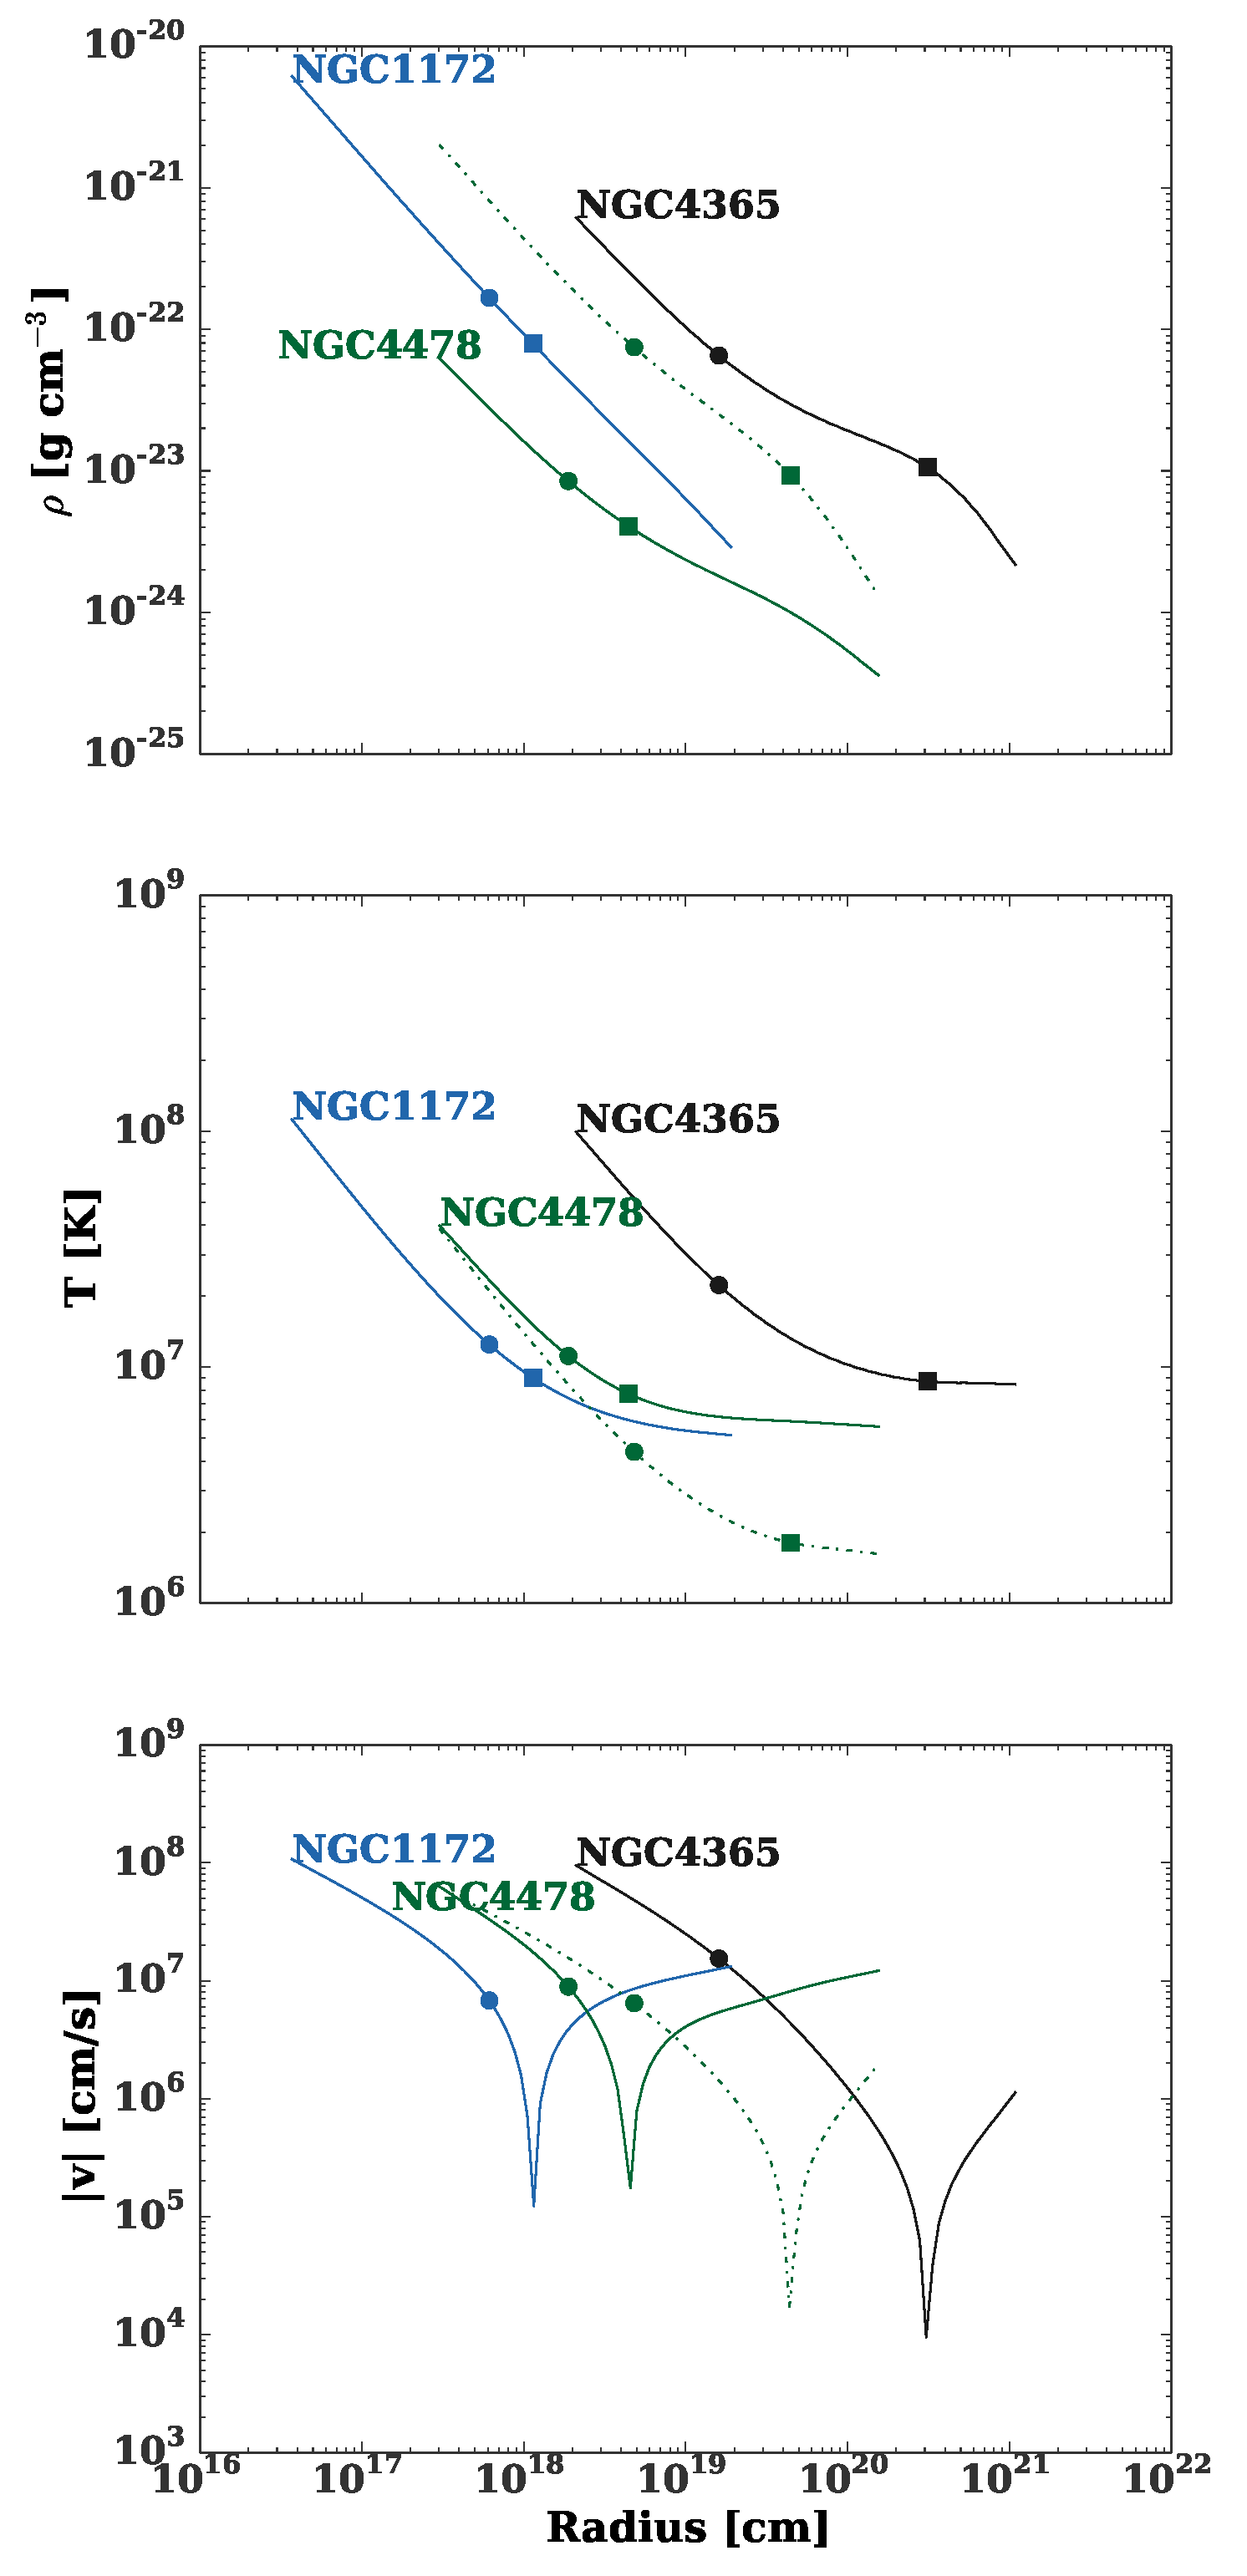
\includegraphics[width=\columnwidth]{profiles.eps}
  \caption{\label{fig:profiles}Radial profiles of the CNM density
    ({\it top}), temperature ({\it middle}), velocity  ({\it bottom}), and
    interior X-ray luminosity ({\it bottom}), calculated for three
    characteristic galaxies from our samples: NGC1172 ({\it blue}),
    NGC4478 ({\it green}), and NGC3115 ({\it black}).  Different line
    styles denote different values of the effective wind heating rate,
    $v_{w,0}$=500 km s$^{-1}$ ({\it solid}) and 200 km s$^{-1}$ ({\it
     dot-dashed}).}
\end{figure}

\begin{figure}
  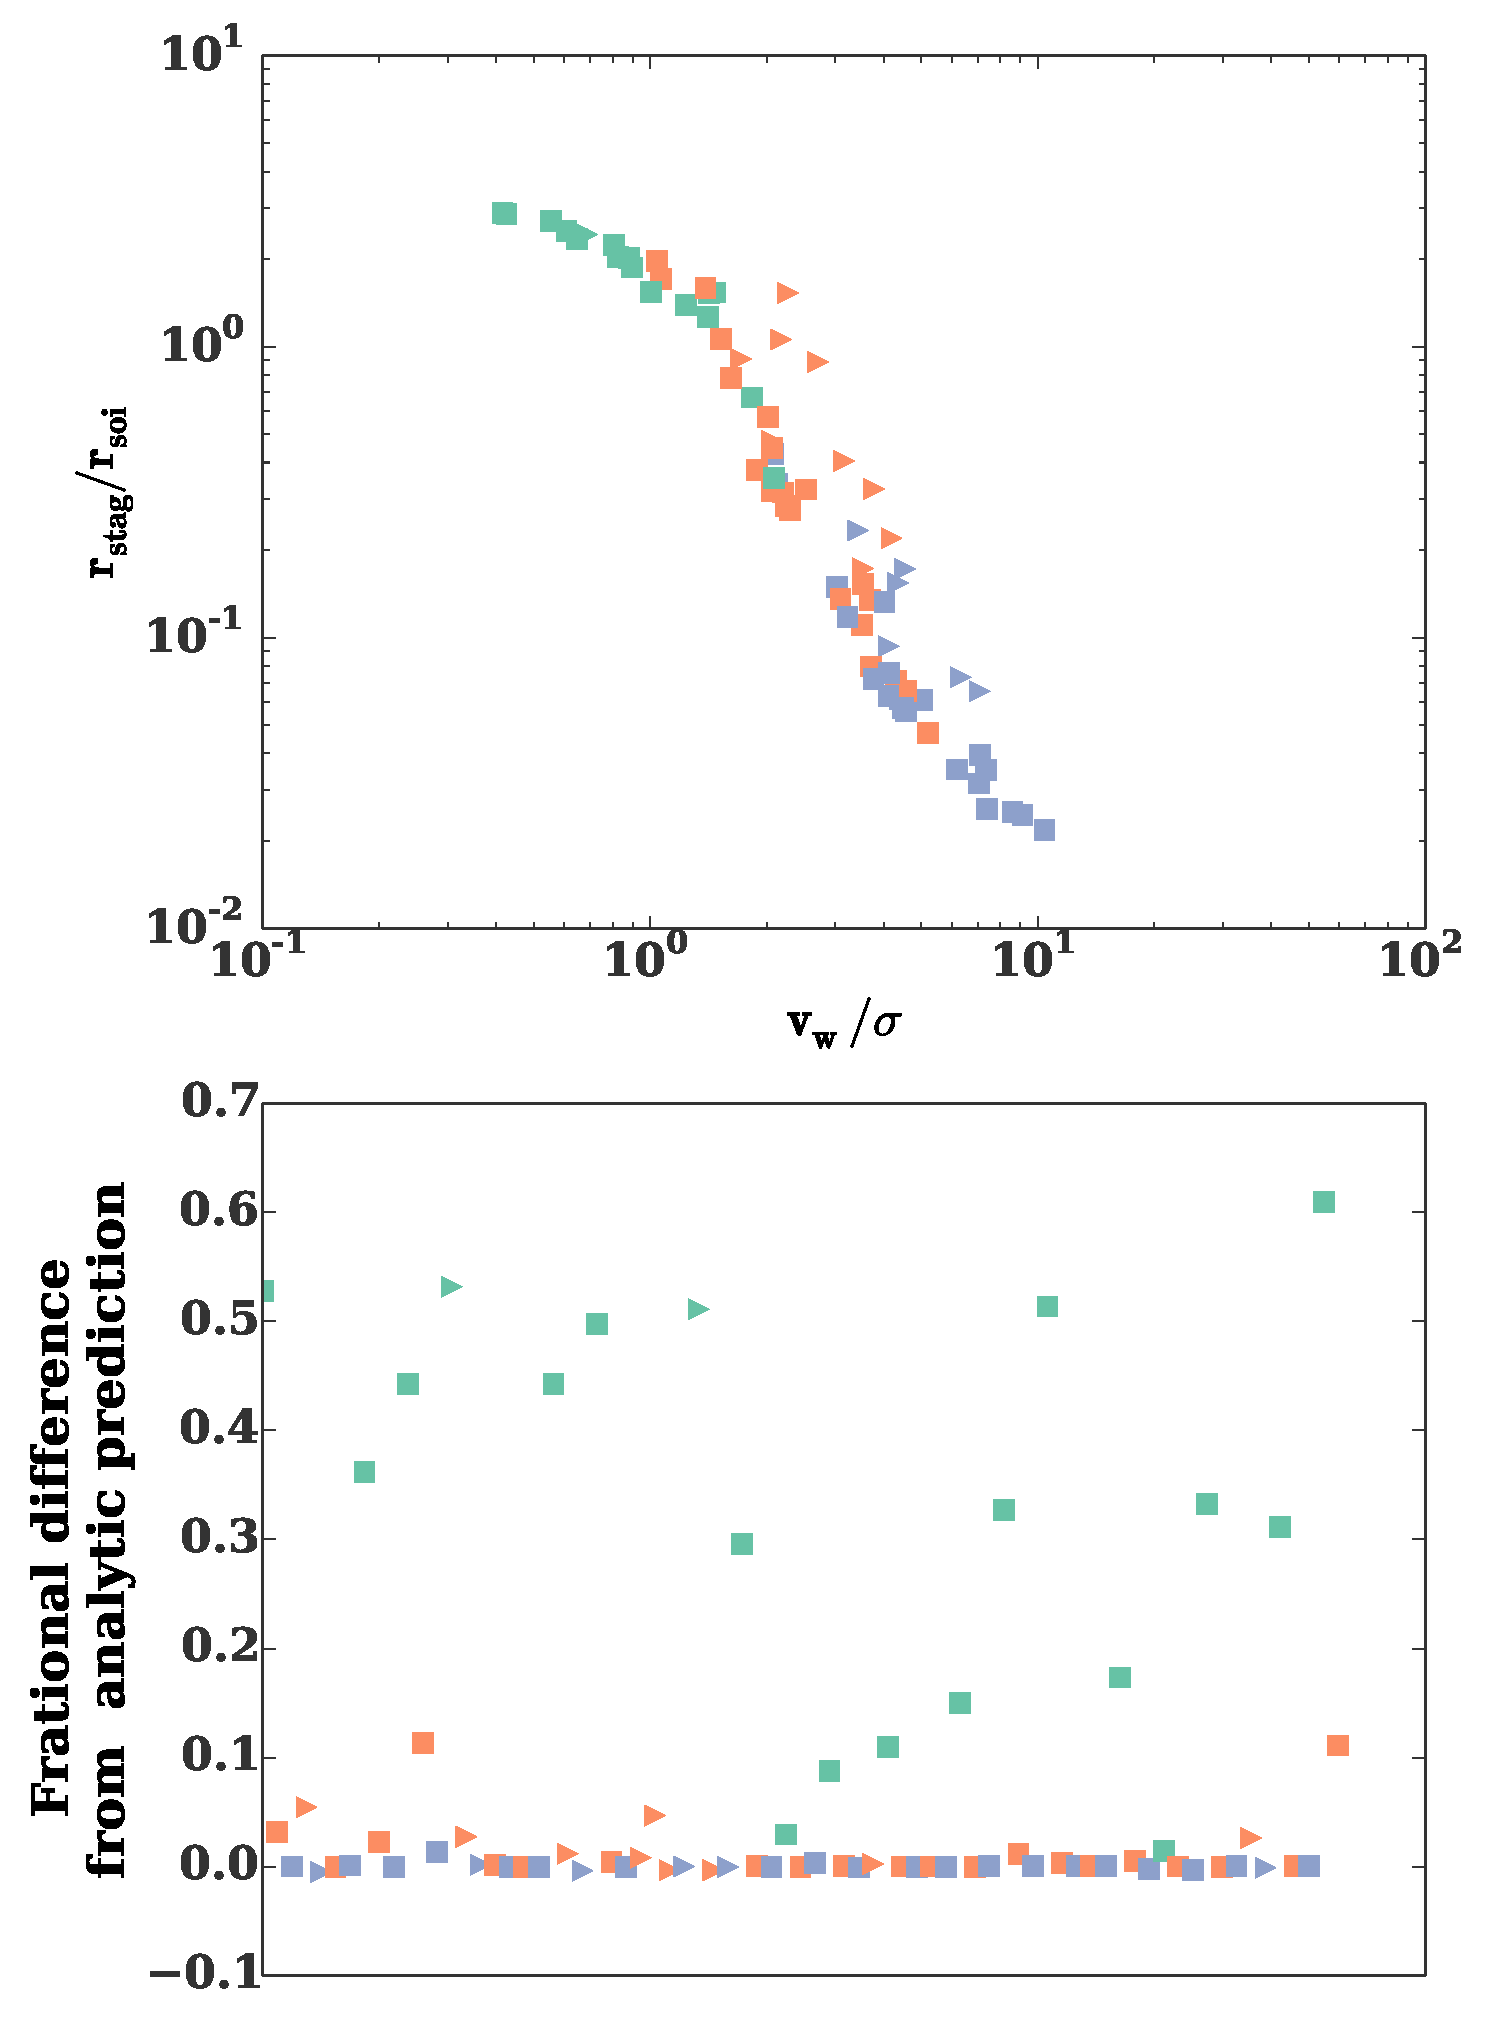
\includegraphics[width=\columnwidth]{rs.eps}
  \caption{\label{fig:stag} \emph{Top panel:} Stagnation radius
    $r_{s}$ (in units of the radius of the sphere of influence $r_{\rm
      soi} = GM_{\bullet}/\sigma^{2}$) for galaxies in our sample as a
    function of the ratio of the effective wind heating rate $v_{w,0}$
    to the stellar velocity dispersion $\sigma$.  Green, orange, and
    blue symbols represent $v_{w,0} =$ 200, 500, and 1000 km s$^{-1}$,
    respectively.  Squares correspond to cusp galaxies, while
    triangles correspond to cores. \emph{Bottom panel}: Fractional
    difference between our numerical calculation of $r_{\rm s}/r_{\rm
      soi}$ and the analytic result in
    equation~(\ref{eq:stag_analytic}). }
\end{figure}



\section{Applications}
\label{sec:applications}
\subsection{Sources of Heating}
\label{sec:heating}

Our results show that the location of the stagnation rate and resulting accretion rate, is very sensitive to the assumed heating
rate $\propto v_{w,0}^{2}$.  Physically, we expect that the heating rate will vary from galaxy to galaxy.. For example, SNe Ia represent a
potentialy important source of heating, but since they are rare they
will only be relevant in a time-averaged sense if the supernova rate
exceeds the inflow time of the gas near the stagnation point.

In this section we discuss potential sources of heating and provide estimates of the value of $\vwO$ corresponding to each.  Before proceeding, note that $\vwO$ is related to the heating rate per volume $e$ according to 
\begin{align}
  &\frac{q \vwO^2}{2}=e \,\,\,\Rightarrow\,\,\,\vwO = \sqrt{\frac{2 t_h e}{\eta \rhostar}}
  \label{eq:vw_eff}
\end{align}

\subsubsection{Stellar winds} Although most of the mass supplied to the CNM by stellar winds occurs during the giant AGB phase, these winds represent a negligible heating source compared to the random wind velocity because the wind velocity $\lesssim 40$ km s$^{-1}$ is much less than the stellar potential $\sigma$.

Main sequence winds, though contributing a much smaller quantity of mass, have much higher velocities and hence contribute a
disproportionally large share of the kinetic energy of winds.  \citet{NaimanSoares-Furtado+:2013a} estimate that $v_{\rm w,0} \sim 100-150$ km s$^{-1}$ for main sequence winds assuming a relatively old stellar population.  On the other hand, for a very young stellar population of age $t_{\star} \lesssim 10^{7}$ yrs the effective wind heating from massive stars can be much greater, $\gtrsim 10^{3}$ km s$^{-1}$.  In what follows below, we take an effective stellar wind heating rate
\be
v_{\rm w,0}^{\star} =  150\,{\rm km\,s^{-1}}
\ee
In Appendix \ref{app:windheat} we present a toy model for how $v_{\rm w,0}$ varies as a function of stellar age ({\bf BDM: Nick can create}).

\subsubsection{Millisecond Pulsars} The spin down power of millisecond
pulsars (MSPs) could in principle be an important heating source.  If
the number of MSPs per unit stellar mass is $n_{\rm msp}$ and each
contributes an average spin-down luminosity $\bar{L}_{\rm sd}$, then the
resulting heating per unit volume $e \approx L_{\rm sd}n_{\rm
  msp}\epsilon$ corresponds to an effective heating rate (eq.~
[\ref{eq:vw_eff}])

  \begin{align}
    v_{\rm w,0}^{\rm p} &=&\left({\frac{2\epsilon t_h n_{\rm msp} \bar{L}_{\rm sd}}{\eta}}\right)^{1/2} \nonumber \\
&\approx&  40\epsilon^{1/2}\left(\frac{\bar{L}_{\rm sd}}{10^{34}\,{\rm erg\,s^{-1}}}\right)^{1/2} \left(\frac{\eta}{0.1}\right)^{-1/2}\,{\rm km\,s^{-1}},
  \end{align}

where $\epsilon< 1$ is the thermalization efficiency of the wind.  The $\sim 30,000$ estimated MSPs in the Milky Way of stellar mass $6\times 10^{10}M_{\odot}$ (\citealt{Lorimer13}) corresponds to $n_{\rm msp}\simeq3 \times 10^{-40} $ MSPs g$^{-1}$, a number we assume in the numerical estimate.  Using the ATNF radio pulsar catalog (\citealt{Manchester+05}), we estimate the average spin-down luminosity of millisecond pulsars in the field (excluding those in globular clusters) to be $\bar{L}_{\rm sd} \sim 10^{34}$ erg s$^{-1}$, in which case $v_{\rm w,0}$ is negligibly small even for $\eta = 0.1$ and $\epsilon = 1$.  

If we assume a higher spin-down luminosity $L_{\rm sd}\simeq 10^{35}$ ergs s$^{-1}$ characteristic of some Fermi pulsars, then we find that $v_{\rm w,0}^{\rm p} \simeq 120\epsilon^{1/2} (\eta/0.1)^{-1/2}$ km s$^{-1}$, in which case MSP heating can be comparable to main sequence wind heating for $\eta = 0.1$, $\epsilon = 1$.  However, much lower thermalization efficiencies of $\epsilon \lesssim 0.1$ are inferred based on modeling the insterstellar mediums of globular clusters \citep{NaimanSoares-Furtado+:2013a}.  Also, the binaries giving rise to MSPs may be disocciated by stellar interactions in the dense nuclear cluster, reducing their numbers as compared to the field population.    
\subsubsection{Type Ia Supernovae} 

Energy injected by Type Ia supernovae (SNe Ia) represents a potentially important source of heating, which unlike core collapse SNe is present even in an evolved stellar population.  Assuming that each Ia injects a thermal energy $E_{\rm Ia}$ into the instellar medium, and that the SNe rate (per stellar mass) is given by $R_{\rm Ia}$, then the resulting volumetric heating rate $E_{\rm Ia}R_{\rm Ia}$ produces an effective wind heating parameter (equation~[\ref{eq:vw_eff}])
\begin{align}
    v_{\rm w,0}^{\rm Ia} =\sqrt{\frac{2 t_h R_{\rm Ia} E_{\rm Ia}}{\eta}} \label{eq:vw_sne}.
\end{align}
The thermal energy injected by a Ia SN $E_{\rm Ia} \simeq \epsilon_{\rm Ia} 10^{51}$ ergs depends on the efficiency $\epsilon$ with which the blast wave energy is converted into bulk or turbulent motion instead of being lost to radiation.  \cite{Thornton+98} estimate a radiative efficiency $\epsilon_{\rm Ia} \sim 0.1$, depending weakly on surrounding density, but \citet{Sharma+14} argues that $\epsilon_{\rm Ia}$ can be considerably higher, $\sim 0.4$, if the SNe occur in a hot dilute medium, as may characterize the CNM.

The Ia SN rate $\RateIa$ depends on the age of the stellar population, as it represent the convolution of the star formation rate and the Ia delay time distribution (DTD) divided by the present stellar mass.  In the limit of impulsive star formation, $\RateIa$ is the DTD evaluated at the time since the star formation episode.  The observationally inferred DTD (Fig. 1 of \citealt{MaozMannucci+:2012a}) has the approximate functional form
\begin{align}
    R_{\rm Ia} =1.7\times 10^{-14}\left(\tau_{\star}/t_{\rm h}\right)^{-1.12} M_{\odot}^{-1}\,{\rm yr^{-1}}
\label{eq:DTD}
  \end{align}
where $\tau_{\star}$ is the time since star formation (c.f.~\citealt{Scannapieco&Bildsten05}).

Using equations (\ref{eq:vw_sne}), (\ref{eq:DTD}), and (\ref{eq:eta}) we thus estimate that
\be
v_{w,0}^{\rm Ia} \approx 250(\epsilon_{\rm Ia}/0.4)^{0.5}(\tau_{\star}/t_{\rm h})^{0.07}\,{\rm km \,s^{-1}},
\ee
showing that the effective velocity due to SN heating is (coincidentally) a weak function of the stellar age.  

The relatively high value of $v_{w,0}^{\rm Ia}$ implies that Ia SNe represent a potentially dominant source of non-AGN heating in the CNM.  However, SNe can only be approximated as "constant" heating source throughout space and time if the rate of SNe is rapid compared to the inflow time at the radius of interest
(\citealt{ShcherbakovWong+:2014a}).  To estimate when this
approximation is valid, we estimate the ``Ia radius"
\begin{align}
r_{\rm Ia} \sim \left(\frac{G}{R_{\rm Ia}\sigma}\right)^{1/2} \sim 38 M_{\bullet,8}^{-0.1}(\tau_{\star}/t_{\rm h})^{0.56}\,{\rm pc} 
\label{eq:rIa}
\end{align}
as the location exterior of which the time interval between subsequent
supernovae $\tau_{\rm Ia} \sim 1/M_{\rm enc}R_{\rm Ia} \sim
G/r\sigma^{2}R_{\rm Ia}$ exceeds the local dynamical timescale $t_{\rm
  dyn} \sim r/\sigma$, where we again adopt the Ia rate for an old
stellar population and in the final equality we estimate the velocity
dispersion using the $M_{\bullet}-\sigma$ relationship
(equation~[\ref{eq:Msigma}]).  Between subsequent supernova, stars release a gaseous mass $M_{\rm gas} \approx \eta M_{\star}\tau_{\rm Ia}/t_{\rm h}$ interior to the Ia radius, which is gravitationally bound to the SMBH by an energy $E_{\rm bind} \approx M_{\rm gas}\sigma^{2}$.  Thus, according to the above definitions, $E_{\rm Ia}/E_{\rm bind} \sim (v_{\rm w,0}^{\rm Ia})^{2}/2\sigma^{2}$.



Note that the stagnation radius scales approximately linearly with $M_{\bullet}$ (equation~[\ref{eq:stag_simple}]), while $\rIa$ is roughly indpendent of SMBH mass.  For small $\Mbh$, the stagnation radius thus lies well inside $\rIa$ and hence Ia SNe will not contribute appreciably to the heating rate.  On the other hand, for massive SMBHs $M_{\bullet} \gtrsim 10^8 \Msun$, SNe Ia  represent an important, and possibly dominant, contribution to the overall heating.

\subsubsection{SMBH Feedback}

Feedback from accretion onto the SMBH also represents a potentially important source of heating which is the most difficult to quantify.  A key difference between AGN heating and other sources discussed thus far is its likely dependence on the mass accretion rate $\dot{M}$.  We assume that the total heating rate from the SMBH is $\epsilon_{\rm j} \dot{M}c^{2}$, where $\epsilon_{\rm j} < 1$ is an efficiency factor.  If this energy is deposited uniformly out to a radius $r_{\rm heat}$ and volume $V_{\rm heat}$, then the local heating rate $e = \epsilon_{\rm j}\dot{M}c^{2}/V_{\rm out}$ results in an effective wind heating rate of
\be
v_w^{\bullet} \approx  \left(\frac{2t_{\rm h}\epsilon_{\rm j}\dot{M}c^{2}}{V_{\rm out}\eta \rho_{\star}}\right)^{1/2} \sim \left(\frac{\epsilon_{\rm j}\dot{M}c^{2}t_{\rm h}}{\eta M_{\rm enc}}\right)^{1/2} \approx c\epsilon_{\rm j}^{1/2}\left(\frac{r_{\rm s}}{r_{\rm heat}}\right)^{\beta/2},
\ee
where we have used the fact that $\dot{M} \approx \eta M_{\rm enc}(r_{\rm s})/t_{\rm h}$ and that $M_{\rm enc}(r) \propto M_{\bullet}(r/r_{\rm soi})^{\beta}$ with $\beta \approx 1-2$ for radii interior to the outer break radius.  Thus for $r_{\rm heat} \sim r_{\rm s}$, even a small heating efficiency $\epsilon_{\rm j} \sim 10^{-6}$ is sufficient for $v_{\rm w,0}^{\bullet}$ to exceed other sources of non-accretion powered heating.  

For a fixed heating radius $r_{\rm heat}$ we just see that $v_{\rm w,0}^{\bullet} \propto r_{\rm s}^{\beta/2} \propto v_{\rm w,0}^{-\beta}$, where in the last proportionality we have used equation (\ref{eq:stag_simple}).  Hence, when SMBH heating dominates, it may ``self-regulate" itself.    

What is a physically motivated value of $r_{\rm heat}$?  \citet{Bromberg+11} show that a jet of luminosity $L_{\rm j}$ and half opening angle $\theta_{\rm j} = 0.1$ (similar to those of AGN jets) propagates through a gaseous mass $M_{\rm g}$ to a radius $r$ in a timescale
\begin{eqnarray}
t_{\rm jet} &\sim& 4000\,{\rm yr}\left(\frac{{L}_{\rm j}}{10^{40}\,\rm erg\,s^{-1}}\right)^{-1/3}\left(\frac{r}{\rm pc}\right)^{2/3}\left(\frac{M_{\rm g}}{10^{8}M_{\odot}}\right)^{1/3} 
\end{eqnarray}
Writing $L_{\rm j} = \epsilon_{\rm j}\dot{M}c^{2}$ and approximating $M_{\rm g} \sim \dot{M}t_{\rm ff}$ we find that the ratio of the jet crossing time to the free-fall time $t_{\rm ff} \sim r/\sigma$ is given by

\begin{equation}
\frac{t_{\rm jet}}{r/\sigma} \sim 8\times 10^{-5}\sigma_{200}^{2/3}\epsilon_{\rm j}^{-1/3},
\end{equation}
which is notably independent of radius $r$.  Thus we require $\epsilon_{\rm j} \gtrsim 10^{-12}$ for the jet to escape, and if it escapes it is free to travel a long distance. 

\subsubsection{Combined Heating Rate} 

The total heating rate $\vwO = \sqrt{v_{\rm w,0}^{\star} + v_{\rm w,0}^{\rm Ia} + v_{\rm w,0}^{\rm p} + v_{\rm w,0}^{\bullet}}$ has contributions from stellar winds, supernovae, pulsars, and SMBH feedback.  Since pulsar heating appears unlikely to contribute appreciably, and since SMBH heating is uncertain, we first focus on heating from stellar winds and supernovae.  

Figure~\ref{fig:vweff} shows an estimate of how the combined heating depends on the age of the stellar population $\tage$ and the SMB mass $\Mbh$.  For $M_{\bullet} \gtrsim 1.5\times 10^8 (\tau_{\star}/t_{\rm h})^{0.5} \Msun$, SNe Ia occur sufficiently frequently within the stagnation radius (i.e., $r_{\rm Ia} > r_{\rm s}$; eq.~[\ref{eq:rIa}]) to contribute their full heating rate.   $v_{\rm w,0}^{\rm Ia} \sim 250$ km s$^{-1}$.  On the other hand, for lower mass BHs Ia SNe are infrequent, in which case main sequence stars ($v_{\rm w,0}^{\star} \simeq 100-150$ km s$^{-1}$) dominate the heating at most times of interest.\footnote{Although SN Ia will still occur surrounding low mass SMBHs, if they are infrequent interior to the radius where the accretion rate is being set, then they will not affect the flow at most near the SMBH at most epochs.}  For very young stellar populations ($\tage \lsim 10^7$ years), $\vwO\simeq 1000$ km s$^{-1}$ due to contributions from line driven winds from high mass main sequence stars.

  \begin{figure}
    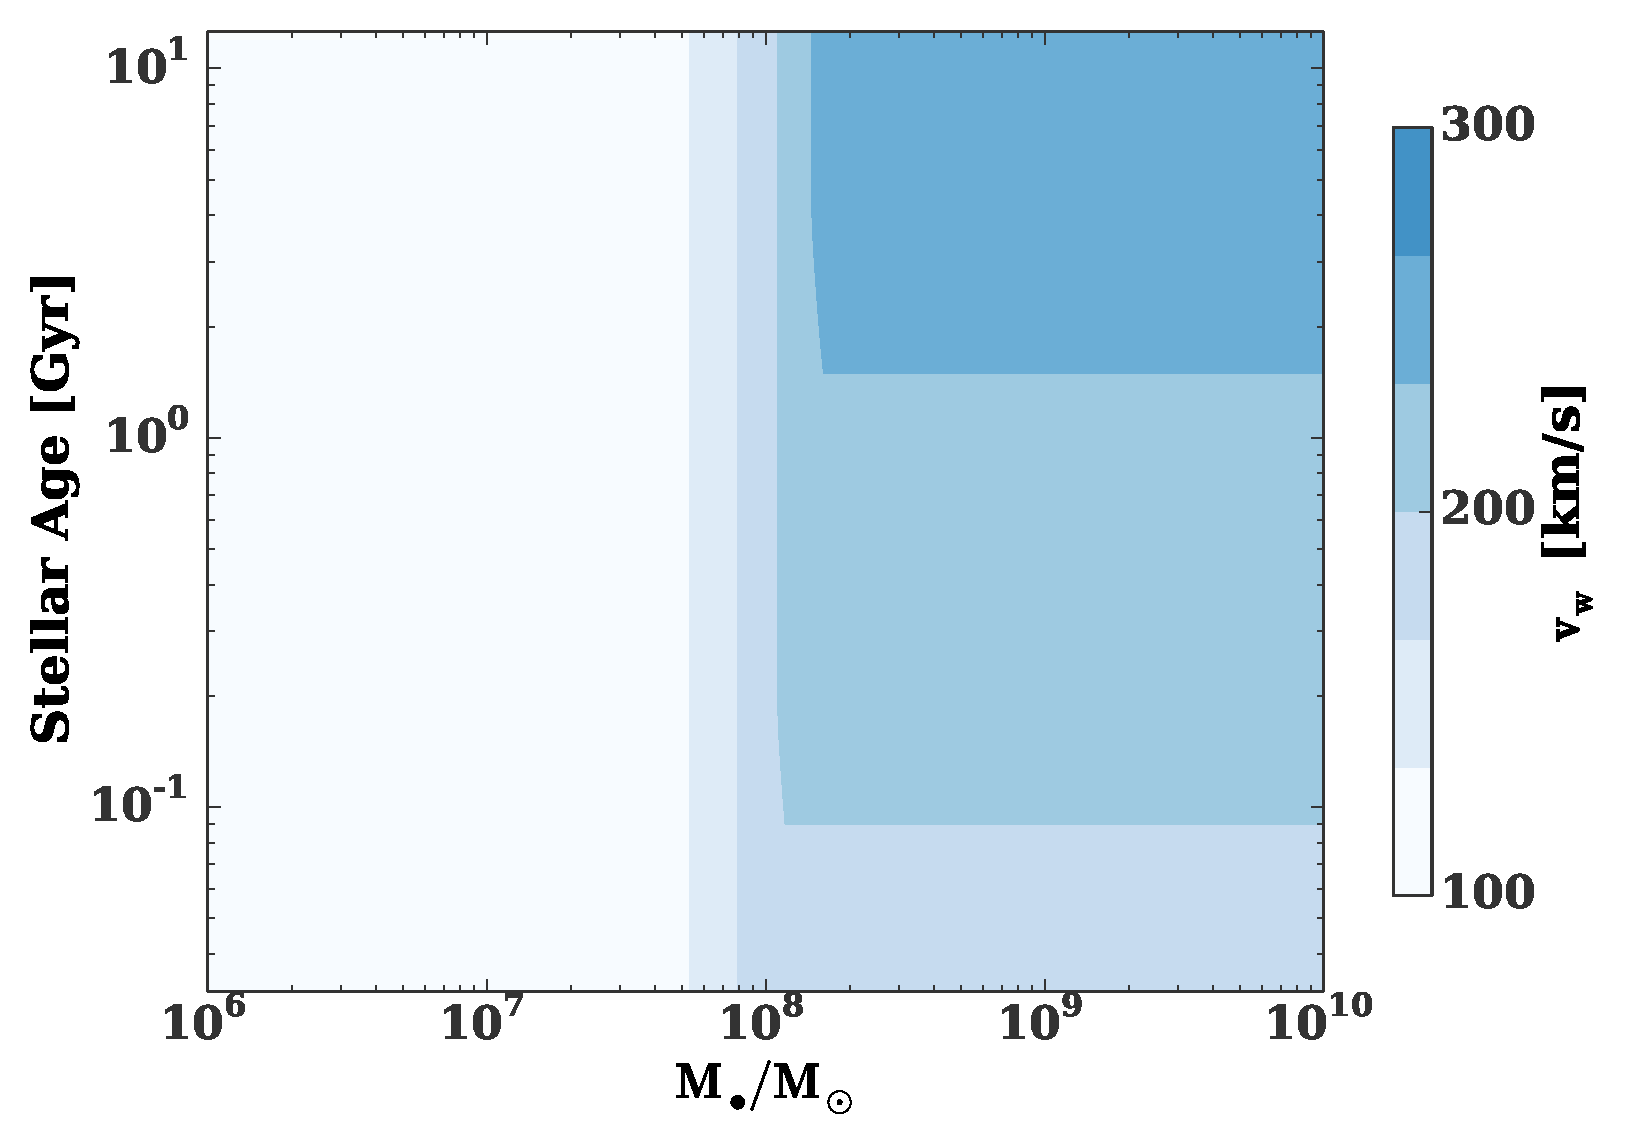
\includegraphics[width=\columnwidth]{vw-contour.eps}
    \caption{\label{fig:vweff} Combined heating rate $\vwO$ of the CNM
      in the parameter space of SMBH mass $\Mbh$ and age of the
      stellar population $t_{\star}$.  We assume that stellar winds
      contribute a constant heating rate $100$ km/s. The contribution
      from SNe Ia is calculated using equation (\ref{eq:vw_sne}), with
      thermalization efficiency $\epsilon_{\rm Ia}=0.4$. The
      contribution from SNe Ia is only added if the $r_s$
      corresponding to the resulting $\vwO$ is outside
      $\rIa$.  {\bf BDM: Correct for dependence of Ia heating on time! among other things}}%describe other cases here.
  \end{figure}

  % AG-I am not comfortable saying type Ia SNe's don't contribute to
  % heating for smaller mass BHs. If the cooling time for the SNe is
  % long then it would be wrong to ignore the SNe contribution. The
  % difference would be that the SNe heating would just be less steady.
  % AG-Thornton and http://arxiv.org/pdf/1402.6695v2.pdf...

\subsection{Mass accretion rate}

For each solution we calculate the accretion rate $\dot{M}$ onto the
SMBH in units of the Eddington accretion rate $\dot{M}_{\rm edd}
\equiv L_{\rm edd}/0.1 c^{2}$, where $L_{\rm edd} \approx 1.4\times
10^{46}M_{\bullet,8}$ erg s$^{-1}$.  Figure~\ref{fig:mdot_mass} shows
$\dot{M}/\dot{M}_{\rm edd}$ as a function of $\Mbh$ for different
values of $\vwO =$ 200, 500 and 1000 km s$^{-1}$.

Note that since we expect $\dot{M}\sim\vwO^{-2}$ for a cusp galaxy and
$\dot{M}\sim\vwO^{-4}$ for a core galaxy
(equation~[\ref{eq:mdot_analytic}]), the mass accretion rate is
expected to be a sensitive function of the assumed heating rate.
However, the accretion rate is proportional to the stellar mass
enclosed inside of $\rs$, so for core galaxies $\dot{M}\sim \Mbh
(\rs/\rsoi)^{2}$,while for cusp galaxies $\dot{M}\sim \Mbh
(\rs/\rsoi)$.  This steeper dependence is enough to offset the
tendency for core galaxies to have a larger $\rs/\rsoi$ for fixed
$\eta$ (see Figure~\ref{fig:stag}). Therefore, for $\rs/\rsoi<1$ core
galaxies would have a smaller $\dot{M}$ than cusp galaxies.  For
$\vwO=1000$ km s$^{-1}$, core galaxies have a smaller accretion rate
for a given SMBH mass.
%% AG-The variation in accretion rate for w/ vw for core galaxies is comparable to that of cusp galaxies and belies the steep dependence stated above.
%% AG-Note separation of cores and cusps (at vw=1000 km/s, where there are enough core galaxies for this comparison to be made). Also, note that the spread in core galaxies is far larger.

We find that $\dot{M}/\dot{M}_{\rm edd}$ tends to increase with SMBH
mass $M_{\bullet}$.  This appears to be in contradiction with the
general down sizing trend observed for SMBH accretion in the local
universe (e.g.~\citealt{Heckman+04}; \citealt{Gallo+08}), such as the
fact that for quiescent galaxies the nuclear X-ray luminosity obeys
$L_X \sim \Mbh^\alpha$, where $\alpha\simeq 0.7-0.8$
\citep{MillerGallo+:2014a}.  Our model instead predicts that $\Mdot
\sim \Mbh^{1.5-2}$, such that if $L_x\sim M$, then we would have $\L_x
\sim \Mbh^{1.5-2}$, steeper than the observed relationship. 

This is shown in the top panel Figure~\ref{fig:bh_xray}. The
relationship from \citealt{MillerGallo+:2014a} and their detection
upper limits are the black and blue solid lines
respectively. The points correspond to the $\dot{M} c^2$ for our
solutions (scaled by $5\times 10^{-7}$).  We must choose a $\vwO$ for
each galaxy.  We select $\vwO$=200 km/s, roughly the expected level of
heating expected from main sequence the stellar winds and MSPs. If
$L_x \sim \Mdot^2$ the discrepancy becomes worse, as shown in the
bottom panel of Fig.~\ref{fig:bh_xray}, where we plot $2 \times
10^{-4} (\eddr) \Mdot c^2$ from our solutions with the relation from
\citealt{MillerGallo+:2014a}.


One possible solution that the wind mass loss rate $\eta$ decreases
with $\Mbh$, as would be expected if low mass SMBH preferentially
hosted older stellar populations.  Another possible explanation is
that the effective heating rate of the CNM $v_{\rm w,0}$ decreases
with decreasing SMBH mass.  This could again be due to an older
stellar population, since $v_{w,0} \propto \eta^{-1/2}$ for heating
sources such as SN Ia and millisecond pulsars.
%, or it could be due to the fact that Ia occur too infrequently inside
%the stagnation radius for low mass black holes.
%AG-We now think that SNe Ia would become important only at the
%highest values of Mbh.
%AG-Note sure where the best place for this discussion would
%be--here or after presenting the comparisons with Miller et al.

\begin{figure}
  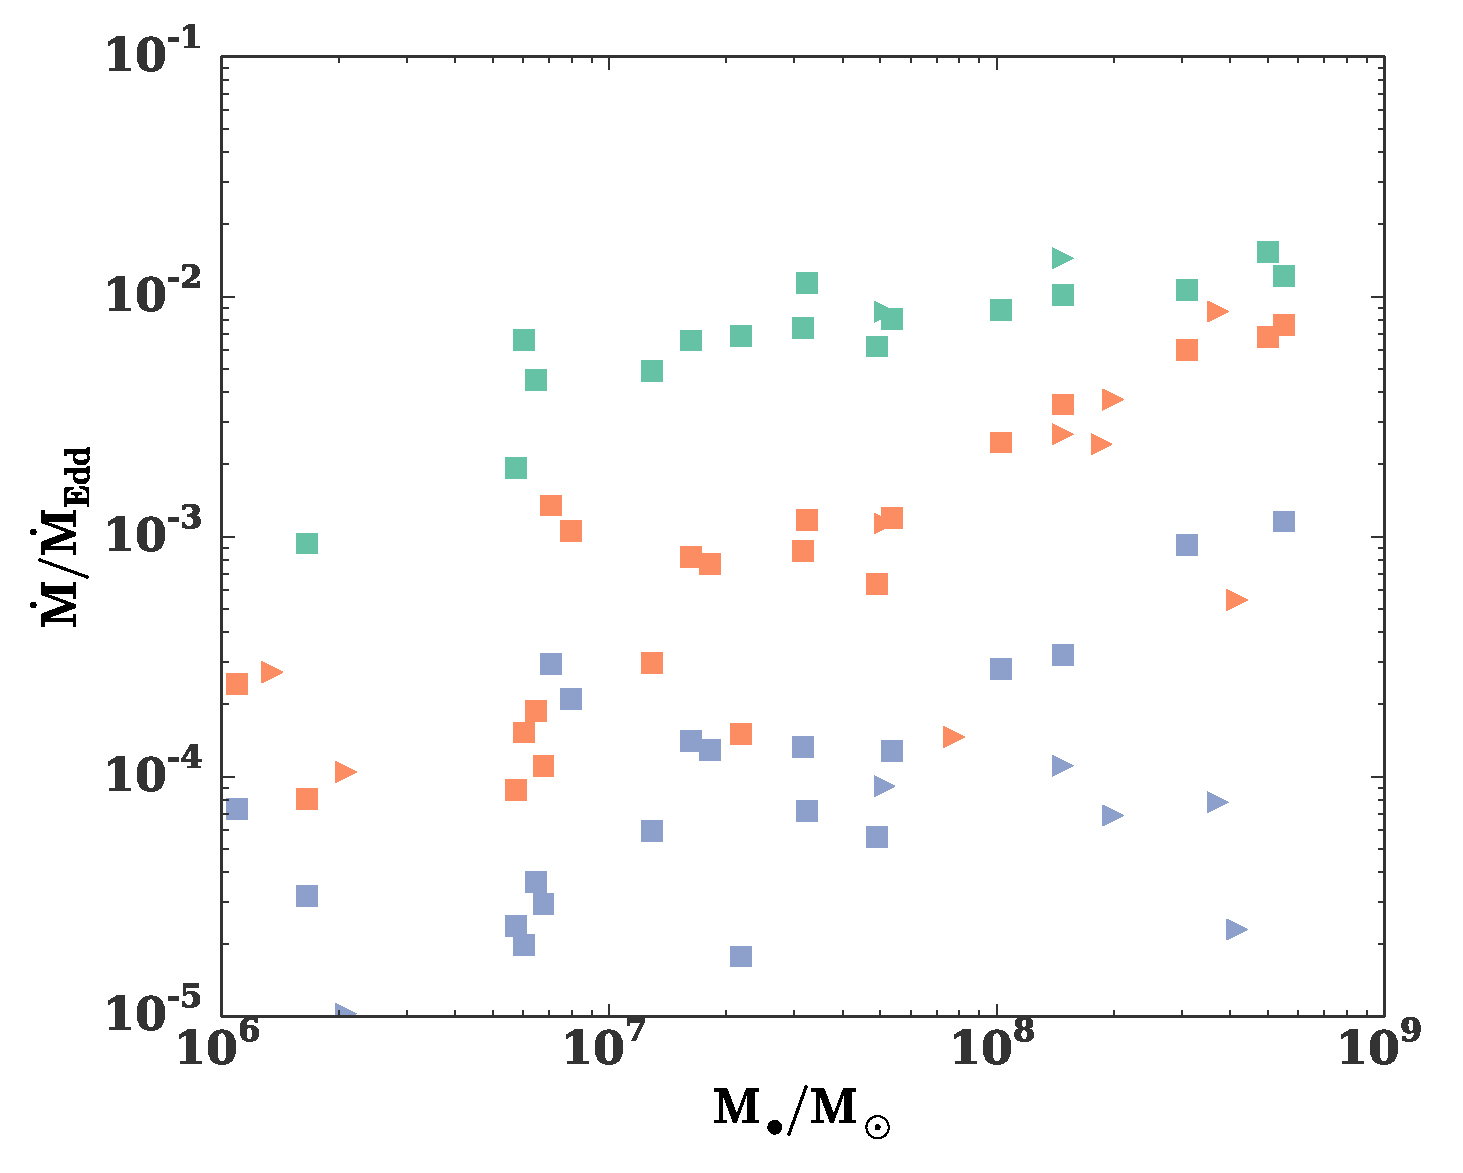
\includegraphics[width=\columnwidth]{mdot_mass.eps}
  \caption{\label{fig:mdot_mass}  Accretion rate $\dot{M}$ in units of the Eddington rate $\dot{M}_{\rm edd}$ as a function of SMBH mass for each galaxy in our sample, calculated for different values of the wind heating parameter $\vwO =$ 200 km s$^{-1}$ ({\it green}), 500 km s$^{-1}$ ({\it orange}), and 1000 km s$^{-1}$ ({\it blue}).  Squares correspond to cusp galaxies, while triangles correspond to cores.}
\end{figure}

%% AG:  Also want to include a plot of x-ray luminosity (less abstract than the accretion rate). 

\subsection{Comparison to Observations}
\subsubsection{Comparison to measured temperature and density profiles}
\citet{AllenDunn+:2006a} use {\it Chandra} X-ray observations to infer the radial temperature and density profiles in the nuclei of nine nearby X-ray luminous elliptical galaxies.  \citet{RussellMcNamara+:2013a} performed a similar analysis with a somewhat enlarged galaxy sample.  Interestingly, these works find a correlation between the accretion rate inferred assuming Bondi accretion and the AGN jet power, which is estimated by the PdV work required to inflate observed cavities in the X-ray emitting gas.  
% At some point it would be useful to describe the differences between
% these two sets of observations \citealt{RussellMcNamara+:2013a}
% tries several different extrapolation schemes for the gas density,
% and finds that that the uncertainty in extrapolating the density
% profile is the dominant source of uncertainty in measuring the
% accretion rate. Find total number which overlaps once the Russell
% galaxies are included...

Five of the galaxies in the \citet{AllenDunn+:2006a} sample overlap with that in \citetalias{WangMerritt:2004a}.  We may thus compare our results for the $T$ and $\rho$ profiles with those inferred from observations for the overlapping galaxies.  The results of this exercise are presented in Fig.~\ref{fig:allen_compare}.

Note that we have two free parameters ($\eta$ and $\vwO$) in our
model, which implies that we can always match the observed temperature
and densities at at least one point.  As a general rule, we find that
a wind heating parameter $\vwO=500$ km s$^{-1}$ gives rough agreement
with the observed temperatures.  We now highlight results for specific
galaxies.
% Thus, we choose $\vwO=500$ km/s.  We choose an
% $\eta$ so that our solution would be consistent with the observed
% density profiles. The comparison is shown in
%% AG-The chosen properties, in particular eta may be summarized in a table.
%% AG-Mention rising temperature profiles on large scales.

\begin{itemize}
% \item \emph{NGC4486} %eta=0.2
%   On scales of $\sim1$ kpc the density profile in
%   \citealt{AllenDunn+:2006a} is shallower than in our model. Our model
%   has a break in the gas density at $\sim 300$ pc--near the location
%   of the Nuker break radius for this galaxy at 560 pc. There is an
%   observed break in the density, but on a scale of a few kpc.

%   The temperature is assumed to be flat from the resolution limit
%   inwards in \citealt{AllenDunn+:2006a}. However, in our models $T$
%   increases monotonically towards the galactic center. This increase
%   is due to the increased velocity dispersion (and thus increased
%   heating) towards the galactic center.

\item \emph{NGC5813} %eta=0.1
  The observed density profile (\citealt{RussellMcNamara+:2013a}) is
  shallower than our calculated density profile, which has a sharp
  break at $\sim$0.1 kpc, the location of the break radius in the
  Nuker profile (this is the radius where the stellar light profile
  transitions from a shallower inner power law slope to a steeper
  outer power law slope).

  For this galaxy we found that we could reproduce the observed
  temperature on large scales with $\vwO=500$ km/s. The increased
  velocity disperision towards the galactic center results in a sharp
  increase in $T$ at small radii, which is not captured in the
  observations due to resolution issues.
\end{itemize}

%It would be nice to have error bars for the observational points in this plot...
\begin{figure*}
  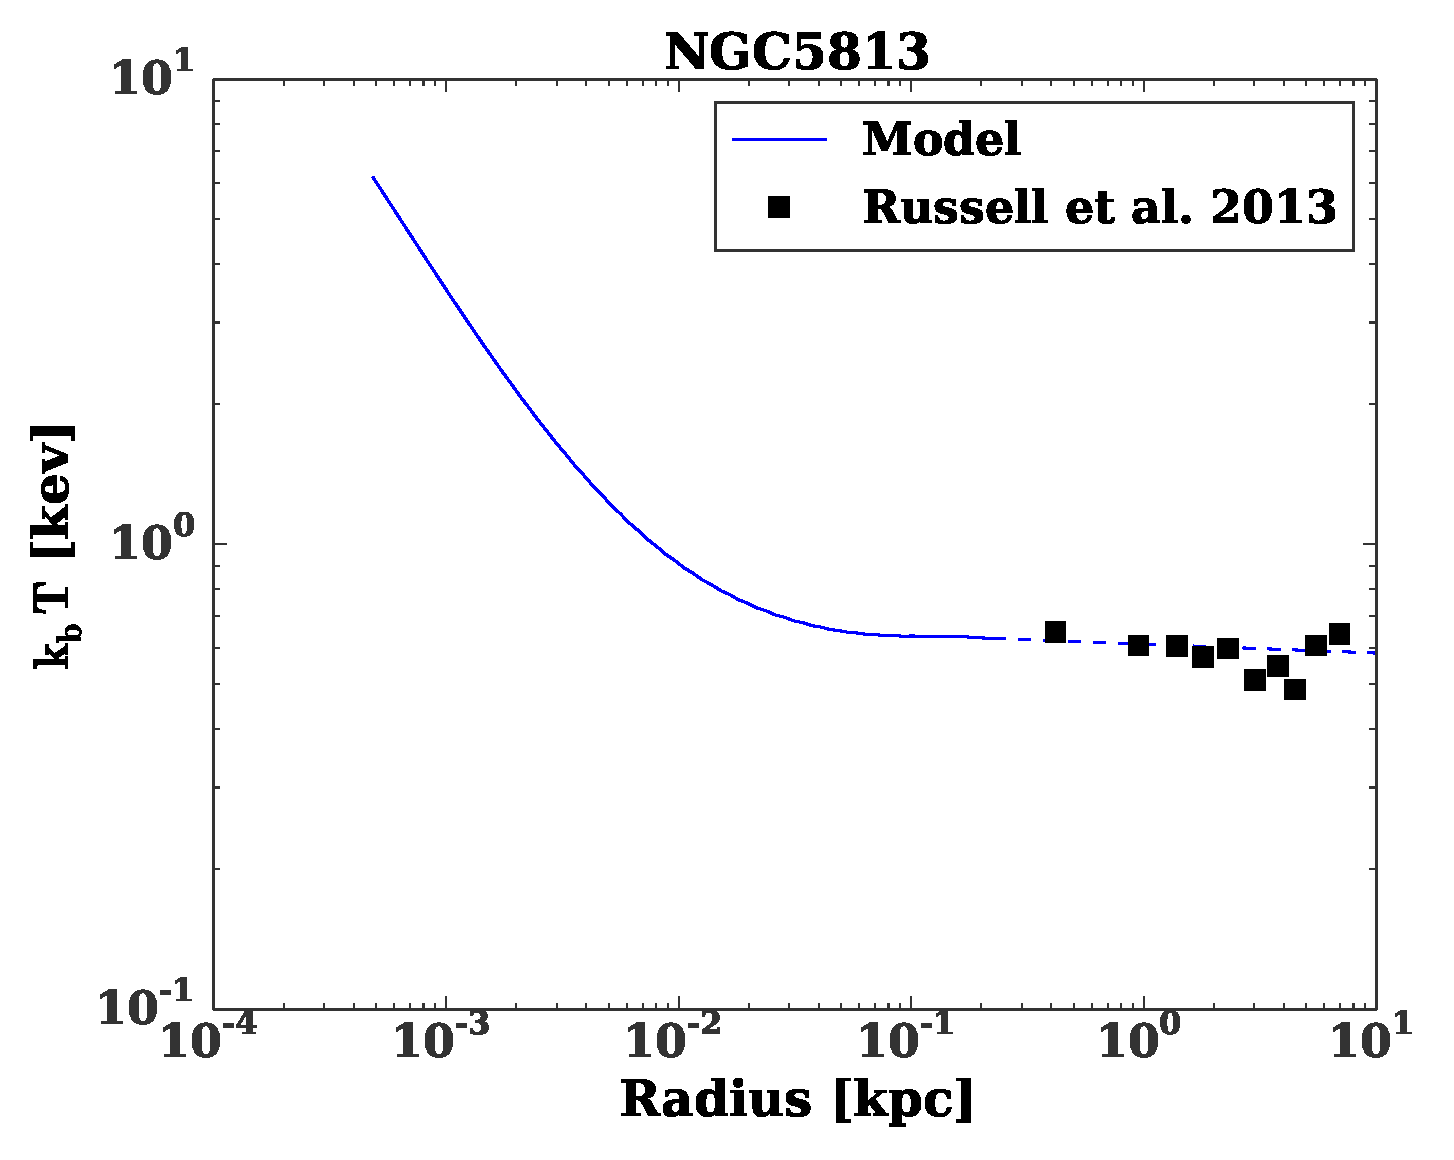
\includegraphics[width=\columnwidth]{NGC5813_T.eps}
  \includegraphics[width=\columnwidth]{NGC5813_rho.eps}
  \caption{\label{fig:allen_compare} Comparison of the radial profiles
    (blue lines) of electron number density $n_e$ and temperature $T$
    to the measured values (black square) in \citet{AllenDunn+:2006a}
    and \citet{ RussellMcNamara+:2013a}. The dashed blue lines are
    power law extrapolations of our profiles. Note that in going from
    $\rho$ to $n_e$ we our adopted value for the molecular weight $\mu=1$.}
  %% AG in the future we will have to be carfeful of the mean molecular weight.
\end{figure*}

% \subsubsection{Comparison with observed X-ray Luminosity-Mass
%   Relation}
% %Note currently I reverse-engineer the stellar mass from the black
% %hole mass inferred from M-sigma; however, it would be better to use
% %the tabulated black hole mass from the Mbh-Mbulge relation.
% Fig. 1 of \citealt{MillerGallo+:2014a} plots the observed
% relationship of unresolved x-ray luminosity versus galactic stellar
% mass for a sample of quiescent galaxies. We may construct a similar
% relationship with our own sample using the inferred accretion rates
% from our solutions.  To infer an x-ray luminosity for each solution,
% we scale our calculated $\Mdot c^2$ by a constant. We pick $5\times
% 10^{-7}$, which gives x-ray luminosities comparable to
% those in \citealt{MillerGallo+:2014a}. We also try an alternate
% prescription in which $L_x$ is quadratic in $\Mdot$. In particular, we
% take $L_x=2 \times 10^{-4} (\eddr) \Mdot c^2$. 

% We must make choose a $\vwO$ for each galaxy.  We select $\vwO$=200
% km/s if $\rs<\rIa$ for this solution, $\vwO$=500 km/s if $\rs>\rIa$
% for this solution, or exclude it.  At low $\Mbh$ we have $\vwO$=200
% km/s and at high $\Mbh$ we have $\vwO$=500 km/s.  Note that much of
% our sample is excluded in this Fig., since for $\vwO$=200 km/s we
% would have $\rs>\rIa$ and four $\vwO$=500 km/s we would have
% $\rs<\rIa$ (i.e. the relative locations of $\rs$ and $\rIa$ would be
% inconsistent with the assumed level of heating).

% %AG-power law may be closer to 1.4 & 1.8 than to 1.5 & 2.
% Our results are plotted in Fig.~\ref{fig:bh_xray}. In our model
% there is a steeper dependence $\Mbh$ on $M_{\rm gal}$ than in
% \citealt{MillerGallo+:2014a}. We find $L_x \propto M_{\rm gal}^{1.5}$ when
% $L_x \propto M_{\rm gal}^{2}$, whereas \citealt{MillerGallo+:2014a} finds
% that $L_x \propto M_{\rm gal}^{0.7-0.8}$. 

\begin{figure}
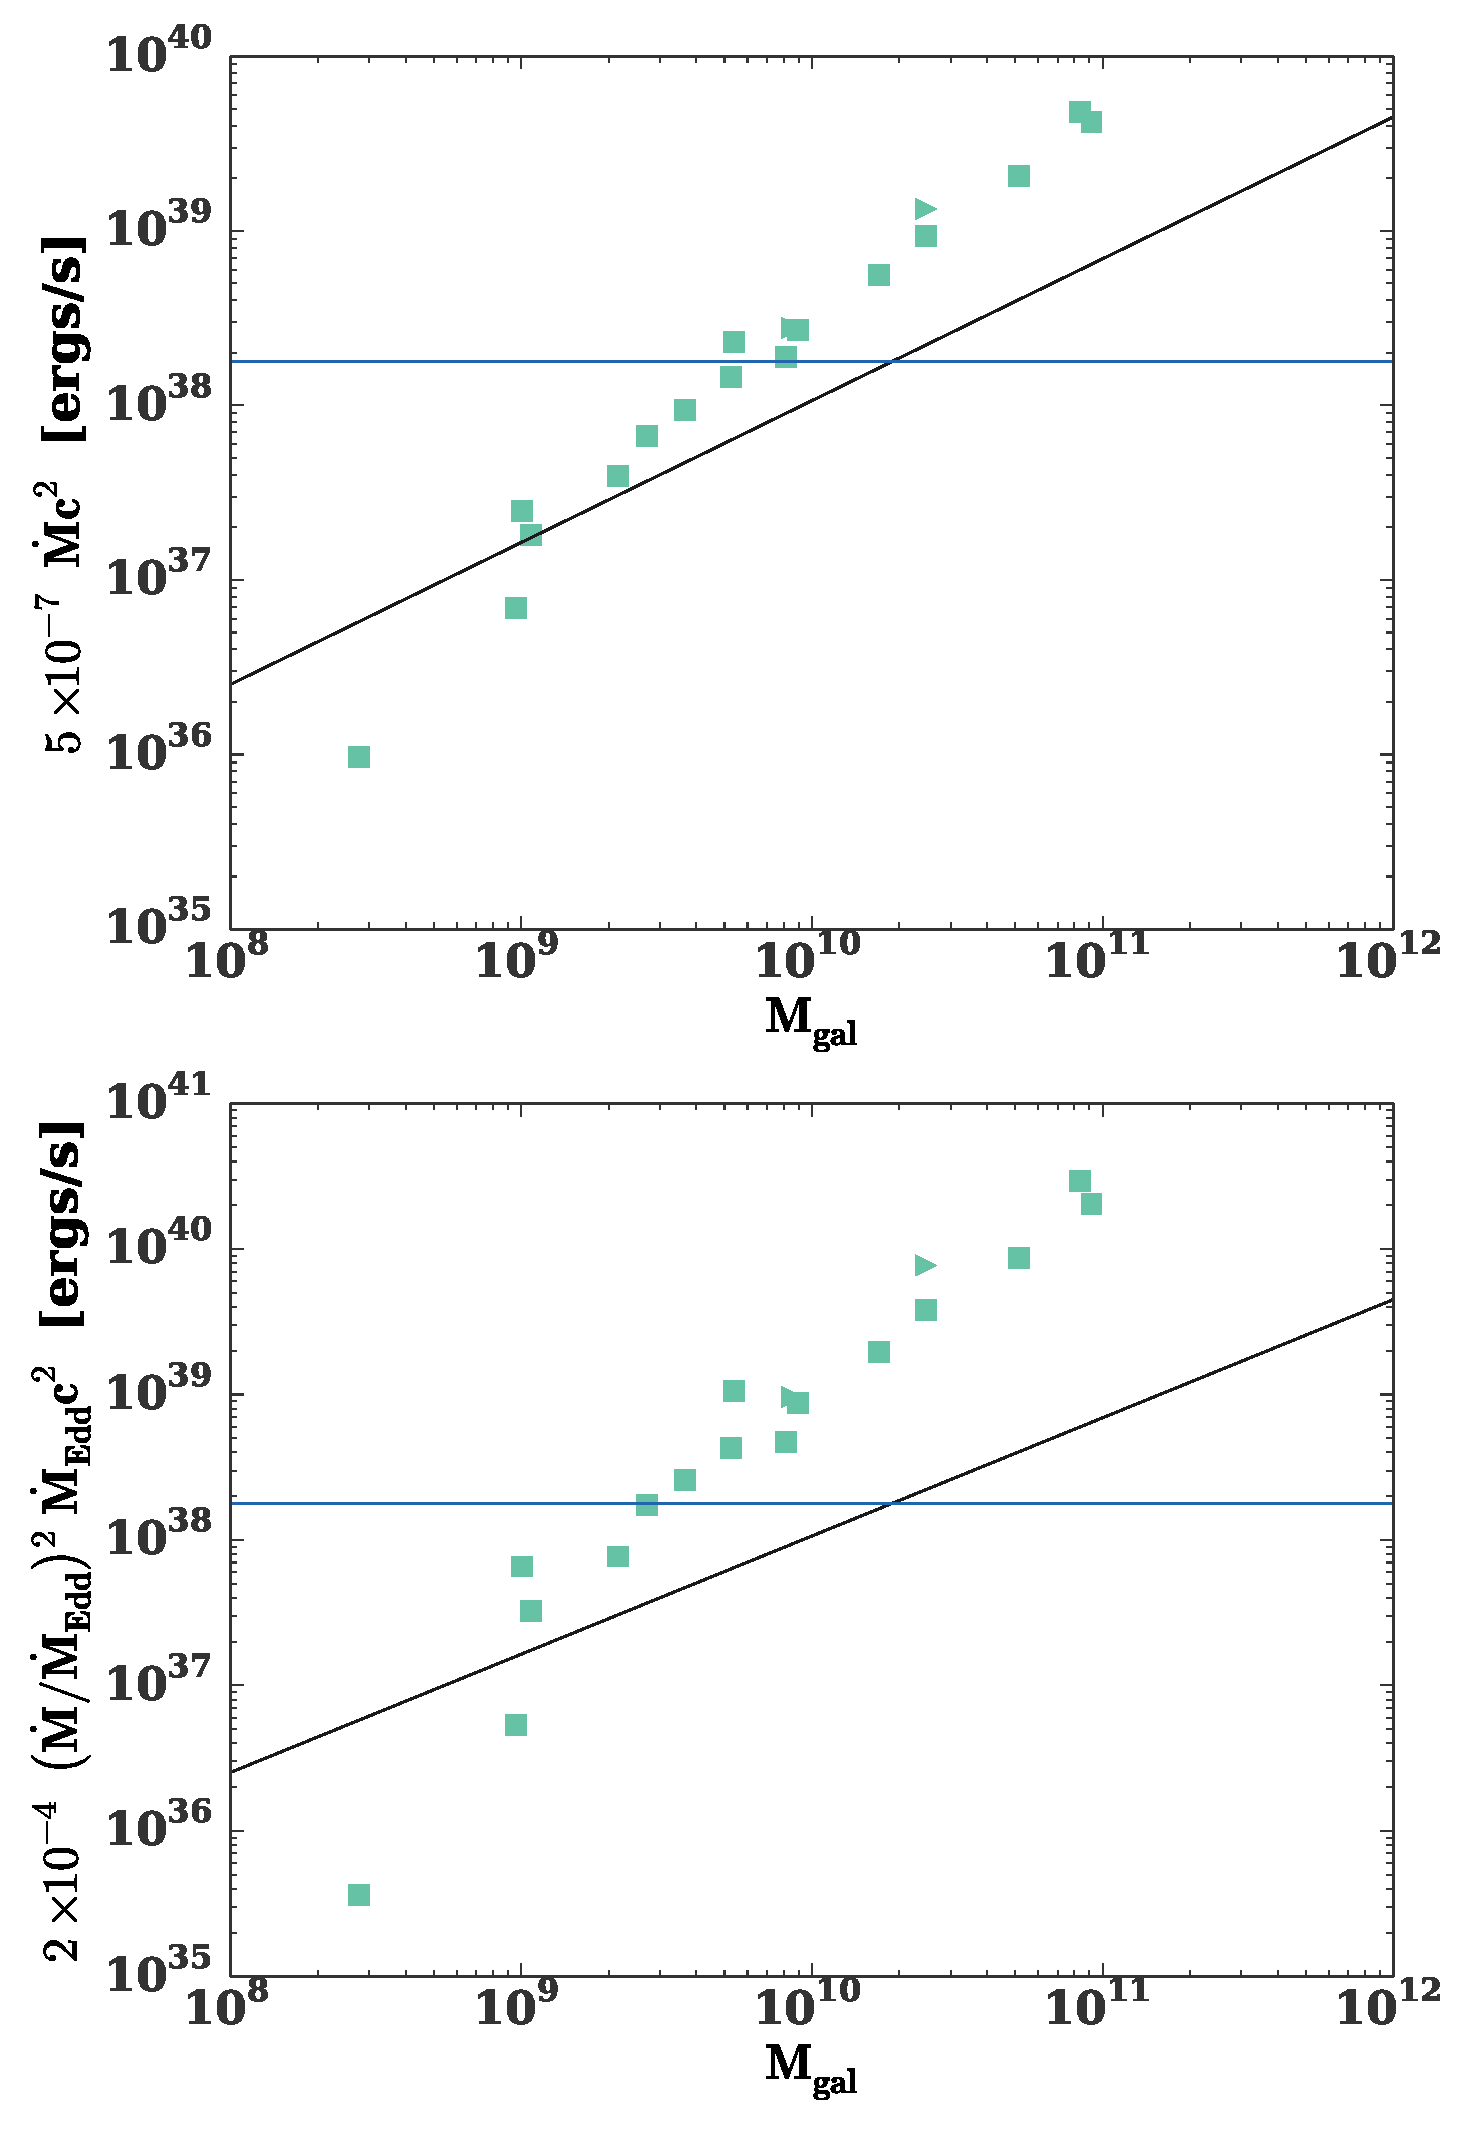
\includegraphics[width=\columnwidth]{bh_xray.eps}
\caption{\label{fig:bh_xray} X-ray luminosity plotted as a function of
  stellar mass for our solutions (points), the trend of nuclear x-ray
  luminosity with stellar mass (black line) and the detection upper
  limit (blue line) from Fig. 1 of \citealt{MillerGallo+:2014a}. In
  the top panel we take the X-ray luminosity to be $\epsilon_1 \Mdot
  c^2$, with $\epsilon_1=5\times 10^{-7}$ chosen to make our
  luminosities comparable to those observed. In the bottom panel, we
  take the accretion power to be quadratic in $\Mdot$. $L_x=\epsilon_2
  \eddr \Mdot c^2$ with $\epsilon2$=$2\times10^{-4}$. For each galaxy
  we choose the $\vwO=200$ km/s solution.  {\bf BDM: if possible, add actual x-ray data from Gallo+08!}}
\end{figure}

\section{Discussion}
\label{sec:discussion}

\subsection{Demographics of SMBHs}

Our analytic expression for the accretion rate (eq.~[\ref{eq:mdot_analytic}]) can be translated into the growth time of the SMBH $t_{\rm grow} \equiv M_{\bullet}/\dot{M}$,
\begin{eqnarray}
  t_{\rm growth}/t_{\rm h} \approx 
  \begin{cases}
    6.3 M_{\bullet,8}^{-0.9}
    v_{500}^{4}  \eta \Msun \, \pyear& \text{core} \\
    2.9 \Mbheight^{-0.4}
    v_{500}^{-2}  \eta \Msun \, \pyear  & \text{cusp}, 
  \end{cases}
  \label{eq:tgrow_analytic}
\end{eqnarray}
which we have normalized in terms of the Hubble time.  

{\bf BDM: ADD plot of parameter space of MBH and stellar age, showing Ia heating versus stellar heating; thermally stable versus unstable regions ($t_{\rm ff} = t_{\rm cool}/10$); as well as where $\sigma = v_{\rm w,0}^{\bullet}$ and $\sigma = v_{\rm w,0}^{\star}$.  }

\subsection{Cooling}
\label{sec:cooling}
Our models neglect radiative cooling, an assumption we now check.  At high temperatures $T\gsim 2\times 10^7$ K gas cools through free-free emission, while at lower temperatures it cools predominantly through metal lines.  To assess the importance of radiative cooling in our solutions we compare the heating rate $H=q \vw^2/2$ to the nominal cooling rate
\begin{align}
  \dot{q}_{\rm cool} =\Lambda(T) n^2,
\label{eq:cooling}
\end{align}
where $n = \rho/\mu m_p$ and we approximate the cooling function $\Lambda(T)$ assuming solar metallicity gas using piece-wise power law (Fig. 34.1 in \cite{Draine:2011a}):
\begin{align}
\Lambda(T)\simeq
  \begin{cases}
    2.3 \times 10^{-24} \left(T/10^6 \text{K}\right)^{0.5} $erg cm$^3 $s$^{-1}&, T \gsim 2 \times 10^7 \text{K} \\
    1.1 \times 10^{-22} \left(T/10^6 \text{K}\right)^{-0.7}  $erg cm$^3 $s$^{-1}&, T \lsim 2 \times 10^7 \text{K}     
  \end{cases}
  \label{eq:cooling2}
\end{align}

If cooling becomes important in the flow, it may lead to thermal instabilities.  There are two kinds of ``instabilities", global and local.  The global instability is simply that, if cooling becomes very rapid, the gas loses thermal pressure and starts to inflow faster, i.e. the entire CNM accretes (e.g.~\citealt{Fabian&Peterson06}).  In practice this should could manifest as a large increase in the stagnation radius, due an effective {\it decrease} in the effective heating rate.  This global ``instability" is not a true instability insofar as the gas does not necessarily clump locally into low-T clouds.  

However, \citealt{McCourt+12} argue that even if cooling is exactly balanced by heating everywhere, there is still a local thermal instability that operates to turn hot gas into cold clouds.  However, this local instability only causes a significant local drop-out of mass from the hot medium (to low-T clouds), if the cooling timescale,
\be
t_{\rm cool} \equiv \frac{3n kT/2}{\dot{q}_{\rm cool}}
\ee 
is locally shorter than the approximately 10 times the free-fall timescale $t_{\rm ff}$. 

Using equations (\ref{eq:Tanalytic}), (\ref{eq:stag_simple}), (\ref{eq:rhors}), (\ref{eq:cooling}), (\ref{eq:cooling2}), we can estimate the ratio of the cooling timescale to the free-fall time $\sim r/\sigma$ at the stagnation radius
\begin{align}
  \left.\frac{t_{\rm cool}}{t_{\rm ff}}\right|_{r_{\rm s}}\simeq
  \begin{cases}
    12 \Mbheight^{-0.66} \eta^{-1}(\chi v_{500})^{6.4}, & \text{core}\\
    6  \Mbheight^{-0.24} \eta^{-1}(\chi v_{500})^{4.4} ,   & \text{cusp}
  \end{cases}
  \label{eq:coolingratio}
\end{align}
We thus see that $t_{\rm cool} \lesssim 10 t_{\rm ff}$ at the stagnation radius for low $v_{\rm w} \lesssim 250$ km s$^{-1}$ if $\eta \sim 0.1$, but even for higher $v_{\rm w}$ if $\eta \sim 1$.    

Fig.~\ref{fig:cooling} shows $t_{\rm cool}/t_{\rm ff}$ as a function of radius for all of our solutions {\bf BDM: change plots}, with different colors denoting different values of $v_{w,0}$.  For our highest heating rates we observe that cooling is unimportant for all solutions across all radii.  With a few exceptions this is also true for $\vwO$=500 km s$^{-1}$.  However, for our lowest heating rate $\vwO$=200 km s$^{-1}$ cooling may be quite important, especially for high $\eta$ (young stellar population;  Appendix~\ref{app:eta}).  

For each of our galaxies Table \ref{tab:eta} provides the maximum value of $\eta$ such that $H/C >$1 at all radii.  Roughly speaking, this is the maximum $\eta$ for which it would be safe to ignore cooling.  If cooling is important, the CNM is likely to be thermally unstable, resulting in the formation of a cold medium that could substantially enhance the rate of accretion onto the SMBH.  

%\begin{align}
 % \Lambda(T)\simeq
  %\begin{cases}
   % 2.3 \times 10^{-24} \left(T/10^6 \text{K}\right)^{0.5} $erg cm$^3 $s$^{-1}& \text{if } T \gsim 2 \times 10^7 \text{K} \\
   % 1.1 \times 10^{-22} \left(T/10^6 \text{K}\right)^{-0.7}  $erg cm$^3 $s$^{-1}& \text{if } T \lsim 2 \times 10^7 \text{K}     
  %\end{cases}
  %\label{eq:cooling}
%\end{align}

\begin{figure}
  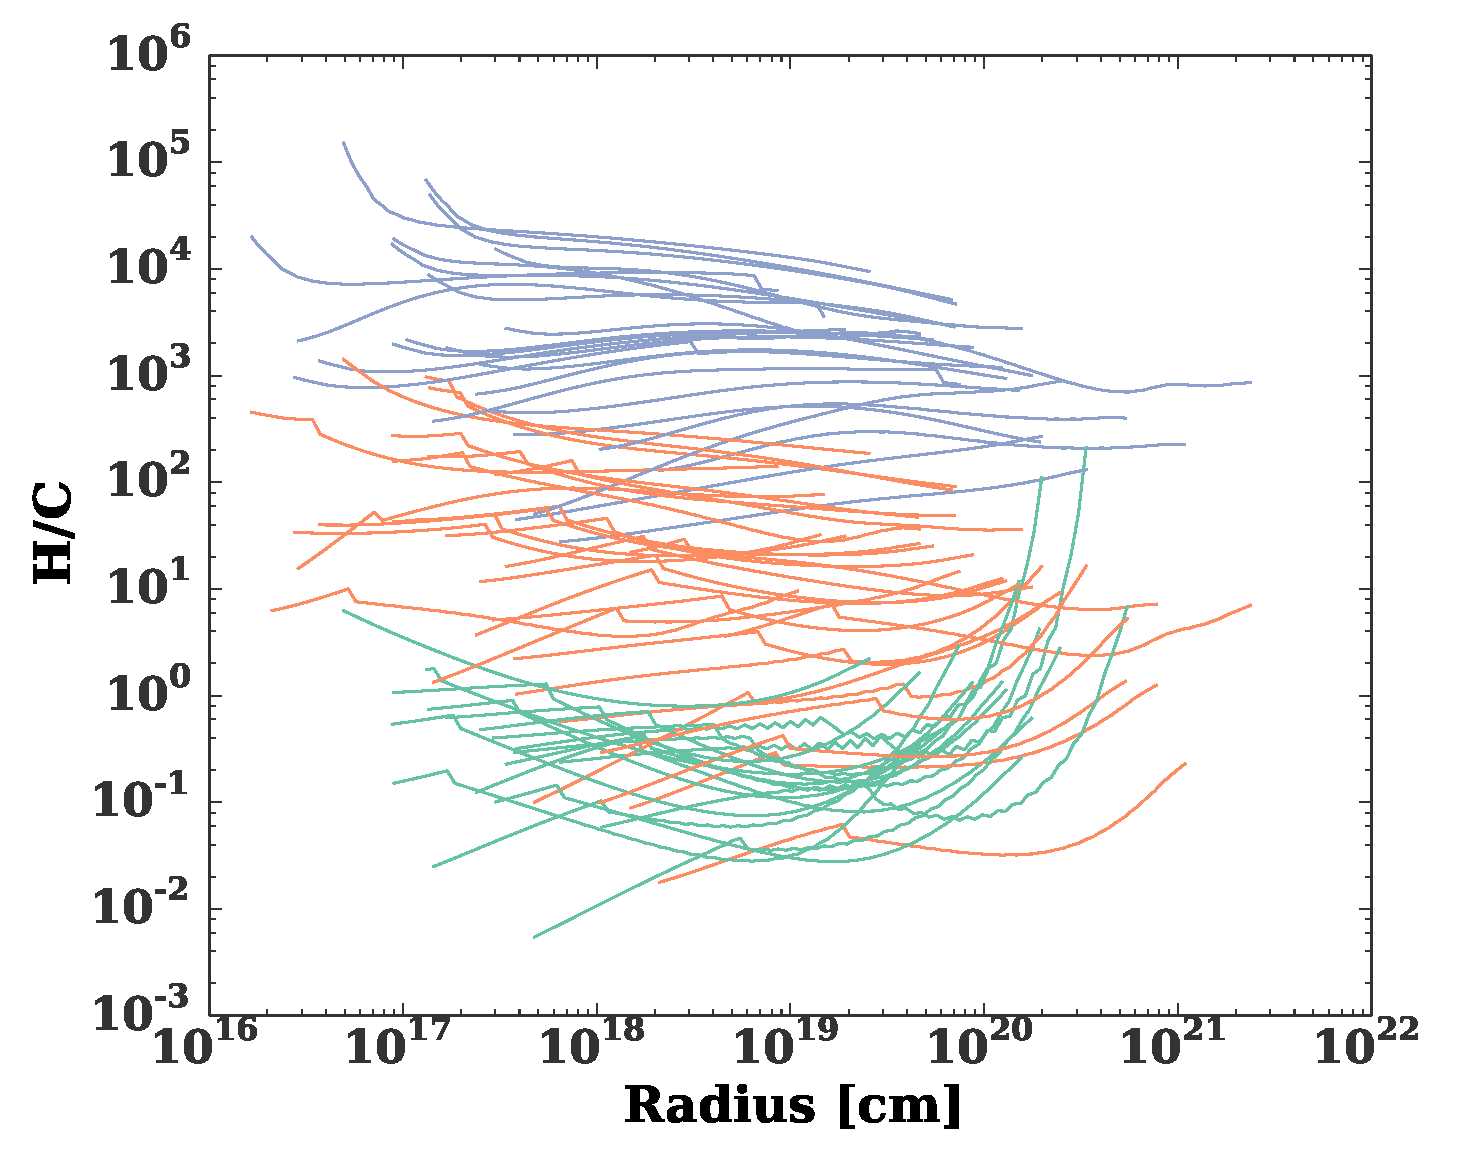
\includegraphics[width=\columnwidth]{cooling.eps}
  \caption{\label{fig:cooling} Ratio of heating ($H$) to cooling rate
    ($C$) for each of our solutions. The cooling rate is calculated
    using the approximate (solar metallicity) cooling function in
    Equation~(\ref{eq:cooling}). The heating rate is estimated as $q
    \vw^2/2$. The ratio is computed from equation (\ref{eq:cooling})
    assuming a stellar mass loss rate parameter $\eta=1$.}
\end{figure}


\input{figures/eta_tab.tex}


  \subsection{Angular Momentum}
  \label{sec:ang}
  Our models are spherically symmetric and do not include the effects of
  the gas' angular momentum. However, galaxies will in general have some
  net rotation, and the gas will generally have some non-zero angular
  momentum. At some radius, $\rcirc$, the specific angular momentum of
  the gas will equal the specific angular momentum of a circular
  orbit. Inside of this radius our assumptions of no rotation and
  spherical symmetry will break down. But if $\rcirc$ is inside of the
  inner sonic point of the flow, the region where angular momentum
  becomes important will be causally disconnected from the rest of the
  flow, and we would be justified in neglecting angular momentum (at
  least on large scales).

  $\rcirc$ depends on the gas injection radius. The largest
  injection radius is $\rs$. Let $\lrs$ be the gas specific angular
  momentum at $\rs$, then 

  \begin{align}
    \rcirc=\frac{\lrs}{G \Mbh}
  \end{align}

  \citet{EmsellemCappellari+:2007a} used two-dimensional kinematic
  data to measure the ratio of ordered to random motion in a sample of
  early type galaxies. More precisely, they measure

  \begin{align}
    \lambda_R=\frac{\left<R|V|\right>}{\left<R\sqrt{V^2+\sigma^2}\right>}
  \end{align}

  Where $R$ is the distance is the distance from the galactic center, $V$ is
  the mean stellar velocity, and $\sigma$ is the velocity
  dispersion. The brackets represent a luminosity weighted average.

  We may rewrite the specific angular momentum at $\rs$ in terms of $\lambda_R$.

  \begin{align}
    \lrs\simeq\lambdars \sigma(\rs)^2 \rs^2
  \end{align}

  Then

  \begin{align}
    \rcirc&\simeq\lambdars^2 \frac{\sigma(\rs)^2}{G \Mbh} \rs^2\\
    &\simeq\lambdars^2 \frac{\rs^2}{\rsoi} \lsim \lambdars^2 \rsoi
  \end{align}

  The inner sonic point, $\rss$ general occurs at $\simeq 1\%$ of
  $\rsoi$. %%AG-Need to explain this somehow.
  So if $\lambdars\lsim 0.1$, $\rcirc<\rss$. In Fig. 2 of
  \citet{EmsellemCappellari+:2007a} $\lambda_R$ is plotted as function
  of radius for a sample of early type galaxies. On scales of $\sim 0.1
  R_e$ $\lambda_R$ is either less than 0.1 or rapidly declining for most
  of their sample %%need to be clearer on rapidly declining also compare
  %% this scale to the sphere of influence scale.
  This suggests that angular momentum should generally be unimportant.

  \section{Summary}
  \label{sec:summary}
  We have calculated steady-state models for circumnuclear medium of a
  sample of early type galaxies, assuming that gas is supplied
  entirely by stellar wind mass loss and heated by shocked stellar
  winds and SNe Ia. We may use these profiles to calculate an $\Mdot$
  onto each of sample galaxy's SMBH, and get the scaling of $\Mdot$
  with $\Mbh$. We may then compare our results with observed trends of
  nuclear x-ray luminosity. Our main conclusions may be summarized as
  follows.

  \begin{enumerate}
  \item We find that $\eddr \propto \Mbh^{\alpha}$, where the value of
    $\alpha$ depends on the slope of the stellar density profile
    ($\alpha\simeq0.5,1$ for cusp and core galaxies respectively). One
    possible solution that the wind mass loss rate (i.e. $\eta$)
    decreases with $\Mbh$, as would be expected if low mass SMBH
    preferentially hosted older stellar populations. Another possible
    explanation is that the effective heating rate of the CNM $v_{\rm w,0}$
    decreases with decreasing SMBH mass. This could again be due to an
    older stellar population, since $v_{\rm w,0} \propto \eta^{−1/2}$
    for heating sources such as SN Ia and millisecond pulsars.
  \item We compare the $\Mdot$ for each of our solution to the one
    calculated from the Bondi formula. We find that they generally to
    a factor of a few. In our model the accretion rate is determined
    from the gas properties at the stagnation radius, $\rs$, which
    agrees with the Bondi radius, $\rb$, within a factor of a
    few. Thus, use of the Bondi formula is a good approximation.
  \item We compare our solutions for density and temperature to those
    inferred from Chandra x-ray observations by \citet{AllenDunn+:2006a}
    and \citet{RussellMcNamara+:2013a} for a handful of galaxies in
    which our sample overlap with theirs. In general, we cannot match
    the observed gas density slope on large scales. 
  \end{enumerate}
  
  \clearpage
  \appendix
  \section{Analytic Expression for the stagnation radius}
  \label{app:rs}
  It is possible to derive an analytic expression for the steady-state
stagnation radius, $\rs$, in terms of $v_w$ and the power law slope of
the density at $\rs$.  Consider the steady-state entropy equation.

\begin{align}
&\rho T v \dsdr=\Q\\
&\dsdr=\frac{\Q}{\rho T v} \label{eq:ss_entropy}
\end{align}

At $\rs$, the velocity, $v$ goes to zero.  Therefore, the numerator
must also go to 0 (otherwise the entropy derivative would blow up at
$\rs$). This implies that

\begin{align}
 &\frac{\gamma}{\gamma-1} \frac{p(\rs)}{\rho(\rs)}=\frac{\vw(\rs)^2}{2} \\
 &\frac{\kb T(\rs)}{\mu \mp}=\gammafi \frac{\vw(\rs)^2}{2} .
\label{eq:appTanalytic}
\end{align}

From the first law of thermodynamics.

\begin{align}
T\dsdr&=\ddr{u}+p\ddr{(1/\rho)}\\
&=\frac{1}{\gamma-1}\ddr{(p/\rho)}-\frac{p}{\rho^2}\ddr{\rho}\\
&=\frac{1}{\gamma-1}\ddr{(p/\rho)}-\frac{p}{\rho} \frac{1}{r} \dxdy{\log{\rho}}{\log{r}} \label{eq:first_law}
\end{align}

Let $n=-\left.d\log(\rho)/d\log(r)\right|_{\rs}$. Combining equation~\ref{eq:ss_entropy} and equation~\ref{eq:first_law},

\begin{align}
\frac{1}{\gamma-1}\left.\ddr{(p/\rho)}\right|_{\rs}+\frac{n}{\rs}  \frac{p(\rs)}{\rho(\rs)}=\left.\underbrace{\frac{\Q}{\rho  v}}_{A}\right|_{\rs} \label{eq:combo1}
\end{align}

The source term on the right may be rewritten using L'Hopital's rule. 

\begin{align}
  &\lim_{r \rightarrow \rs} A=\frac{\lim_{r \rightarrow \rs}
    \frac{d}{dr}\left[q (r)\left(\ke -\gammaf
        \frac{p}{\rho}+\kew\right)\right]}{\lim_{r \rightarrow \rs}
    \frac{d}{dr} \left(\rho v\right)}\\
  &=\frac{ q'(\rs) \overbrace{\left.\left(\ke
        -\gammaf\frac{p}{\rho}+\kew\right)\right|_{\rs}}^0+ q(\rs)
    \frac{d}{dr} \left[\left(\ke -\gammaf
        \frac{p}{\rho}+\kew\right)\right]_{\rs}}{\underbrace{\rho'(\rs)
      v(\rs)}_0 +\underbrace{v'(\rs)\rho(\rs)}_{q(\rs)}}\\
  &= \frac{d}{dr} \left[\left(\ke -\gammaf \frac{p}{\rho}+\kew\right)\right]_{\rs}
\end{align}

$\vw^2=\vwO^2+ G \Menc/r$, where
$\Menc=\Mbh+\Mstar$. Assuming $\Mstar \sim r^{2-\Gamma}$,

\begin{align}
\lim_{r \rightarrow \rs} A=-\gammaf
\left.\ddr{(p/\rho)}\right|_{\rs}-\frac{G \Menc(\rs)}{2 \rs^2}+(2-\Gamma) \frac{G
  \Mstar(\rs)}{2 \rs^2}.
\end{align}

Substituting this expression back into Eqn. (\ref{eq:combo1})

\begin{align}
&\frac{\gamma+1}{\gamma-1}
\left.\ddr{(p/\rho)}\right|_{\rs}+\frac{n}{\rs}
\frac{p(\rs)}{\rho(\rs)}=-\frac{G \Menc(\rs)}{2 \rs^2} + (2-\Gamma) \frac{G
  \Mstar(\rs)}{2 \rs^2}.  \label{eq:rs1}
\end{align}

At the stagnation point we also have (from the momentum equation)

\begin{align}
&\frac{1}{\rho}\dpdr=- \frac{G\Menc}{\rs^2}\\
&\ddr{(p/\rho)}-p \ddr{(1/\rho)}=-\frac{G \Menc}{\rs^2}\\
&\ddr{(p/\rho)}+\frac{p}{\rho^2} \ddr{\rho} = -\frac{G \Menc}{\rs^2}\\
&\ddr{(p/\rho)}+\frac{p}{\rho}
\underbrace{\frac{d\log(\rho)}{dr}}_{-n/r} = -\frac{G \Menc}{\rs^2} \label{eq:HSE}
\end{align}

Combining equation (\ref{eq:rs1}) and equation (\ref{eq:HSE}) 

\begin{align}
&2 n \gammaf \frac{p(\rs)}{\rho(\rs)}= A \frac{G \Mstar(\rs)}{\rs} +B \frac{G \Mbh}{\rs}\\
&A=\left[\frac{4\gamma-(\gamma-1)(1+\Gamma)}{2 (\gamma-1)}\right]\\
&B=\frac{\gamma+3}{2 (\gamma-1)}
\end{align}

Then using equation (\ref{eq:appTanalytic})

\begin{align}
& \rs=\frac{G \Mbh}{n \vw(\rs)^2}\left(A \frac{\Mstar(\rs)}{\Mbh} +B\right).
\end{align}

Let  $\eta=v_{w,0}/\sigma_{\rm soi}$. We
may re-parameterize this relationship as follows:

\begin{align}
  \x=\frac{1}{\zeta^2 n}\left[
   \frac{\Mstar(\rs)}{\Mbh}\left(A-\frac{n}{2}\right)+\left(B-\frac{n}{2}\right)\right].
\end{align}

Note that in general $\omega$ is an implicit function of $x$. Cusp galaxies have $\Gamma\simeq1$.  Then $\Mstar(\rs)/\Mbh=x$. With $\gamma=5/3$, $A=2$ and $B=7/4$.  Then:

\begin{align}
\x=\frac{7-2n}{2\zeta^2 n+2n-8}
\end{align}

Consider the limit $\lim_{\eta \to 0}$ (the extra heating $\vwO$ goes to 0. Then we will get a negative value for the stagnation radius unless the gas density profile is quite steep at the $\rs$: $3.5<n<4$.

In contrast for a core galaxy we will have $\Gamma\simeq0, A=9/4,
B=7/4$, and $\Mstar/\Mbh=x^2$. Thus we will have a quadratic equation for
stagnation radius, which gives

\begin{align}
\x=\frac{\zeta^2 n \pm \sqrt{\eta^4 n^2 -4 \left(\frac{9}{4}-\frac{n}{2}\right) \left(\frac{7}{4}-\frac{n}{2}\right)}}{2\left(\frac{9}{4}-\frac{n}{2}\right)}
\label{eq:rstag}
\end{align}

Consider the limit $\lim_{\zeta \to 0}$, then for $\rs$ to exist we must have $3.5<n<4.5$.

When $\Mstar << \Mbh$ at the stagnation radius, the relationship between $\rs$ and $\vw$ is greatly simplified. 

\begin{align}
\kewO=\frac{7}{4}\frac{G \Mbh}{n \rs}
\end{align}

Where the pre-factor on the right-hand side is valid for $\gamma=5/3$ and $\Gamma=1$ or 0.  

%%% Local Variables:
%%% mode: latex
%%% TeX-master: "ms"
%%% End:



  \section{Analytic model for dependence of wind mass loss rate on stellar age}
  \label{app:eta}
  \input{eta}

\section{Analytic model for dependence of wind heating $v_{\rm w,0}^{\star}$ on stellar age}
\label{app:windheat}
{\bf BDM: Nick add}
  \footnotesize{
    \bibliographystyle{mn2e}
    \bibliography{master}
  }
\end{document}
